%# -*- coding: utf-8-unix -*-
%%==================================================
%% thesis.tex
%%==================================================

% 双面打印
%\documentclass[doctor, fontset=adobe, openright, twoside, zihao=-4]{sjtuthesis}
 \documentclass[bachelor, fontset=adobe, openany, oneside, zihao=-4]{sjtuthesis} 
% \documentclass[master, adobefonts, review]{sjtuthesis} 
% \documentclass[%
%   bachelor|master|doctor,	% 必选项
%   fontset=adobe|windows,  	% 只测试了adobe
%   oneside|twoside,		% 单面打印,双面打印(奇偶页交换页边距,默认)
%   openany|openright, 		% 可以在奇数或者偶数页开新章|只在奇数页开新章(默认)
%   zihao=-4|5,, 		% 正文字号:小四、五号(默认)
%   review,	 		% 盲审论文,隐去作者姓名、学号、导师姓名、致谢、发表论文和参与的项目
%   submit			% 定稿提交的论文,插入签名扫描版的原创性声明、授权声明 
% ]

\begin{document}

%% 无编号内容:中英文论文封面、授权页
%# -*- coding: utf-8-unix -*-
\title{基于多模态深度自编码器情绪识别研究}
\author{付\quad{}豪}
\advisor{吕宝粮教授}
% \coadvisor{某某教授}
\defenddate{2016年6月14日}
\school{上海交通大学}
\institute{计算机科学与工程系}
\studentnumber{5120309235}
\major{计算机科学与工程}

\englishtitle{Multi-modal Deep Auto-encoder Based Emotion Recognition}
\englishauthor{\textsc{Hao Fu}}
\englishadvisor{Prof. \textsc{Bao-liang Lu}}
% \englishcoadvisor{Prof. \textsc{Uom Uom}}
\englishschool{Shanghai Jiao Tong University}
\englishinstitute{\textsc{Depart of Computer Science and Engineering, School of SEIEE} \\
  \textsc{Shanghai Jiao Tong University} \\
  \textsc{Shanghai, P.R.China}}
\englishmajor{Computer Science and Engineering}
\englishdate{Jun. 14th, 2016}


\maketitle

\makeenglishtitle

\makeatletter
\ifsjtu@submit\relax
	\includepdf{pdf/original.pdf}
	\cleardoublepage
	\includepdf{pdf/authorization.pdf}
	\cleardoublepage
\else
	\makeDeclareOriginal
	\makeDeclareAuthorization	
\fi
\makeatother


\frontmatter 	% 使用罗马数字对前言编号

%% 摘要
\pagestyle{plain}
%# -*- coding: utf-8-unix -*-
%%==================================================
%% abstract.tex for SJTU Master Thesis
%%==================================================

\begin{abstract}
随着计算机的发展,我们期望能用一种高效而且准确的方法识别人类的情绪,从而在人机交互与人人交互中发挥巨大的作用。在基于各种信号的情绪识别中,基于脑电信号的情绪识别算法由于与激发情绪的大脑活动有直接关联,无疑成为当前最有可能获得较高准确度的情绪识别算法之一。因此,建立一套能广泛适用于不同个体之间的算法模型有着非常重要的实际意义,也成为当下基于脑电信号的情绪识别研究的热点之一。与此同时,随着机器的计算能力的提高,深度学习的方法例如卷积神经网络,深度置信网络,深度自编码器等受到研究人员的青睐。但是如果只是用单一模态的输入进行学习,由于数据的分布总是相似的,所以提供的信息和学习能力都是很有限的。相反,不同模态譬如声音,文字,图像,脑电,眼动轨迹带有不同信息,所以提供的数据分布各不相同,他们各自提供的信息不但有交集,还互相补充。因此,如果能够利用多模态输入信号的融合,我们不仅可以提取出多模态共有的特征表达,从而找出它们代表的现实世界中的意义,还可以利用多个模态不同信号的互补信息来提高情绪识别任务的准确率。

\keywords{\large 深度学习 \quad 深度自编码器 \quad 多模态 \quad 互补特征}
\end{abstract}

\begin{englishabstract}

	With the development of computers, we can expect an efficient and accurate method of identifying human emotions, which play a huge role in human-computer interaction and human interaction in. In the emotion recognition based on various signals, emotion recognition algorithm based on brain electrical signal due to excitation emotional brain activity directly related, it will undoubtedly become one of the most likely to get the emotion recognition algorithm high accuracy. Therefore, the establishment of a widely applicable model algorithm has a very important practical significance between different individuals, it has become one of the hot emotion recognition based on the current EEG. In the meantime, with the improvement of the machine's computing power, depth of learning methods such as convolution neural network, the depth of belief networks, since the depth encoder favored by researchers. However, if only a single mode input learning, since the distribution of the data is always similar, so the ability to provide information and learning are very limited. Instead, different modalities such as voice, text, image, EEG, eye movement trajectory with different information, so the data provided by each of the distribution are not identical, they each provide information not only joy, but also complement each other. Therefore, if harnessed fusion multimodal input signal, we can extract only feature common to multi-modal expression, to find out the real world in the sense that they represent can also use complementary information of a plurality of signals of different modes to improve the accuracy of emotion recognition task.
	
\englishkeywords{\large Deep learning \quad Deep auto-encoder \quad multi-modal \quad feature-complement}
\end{englishabstract}



%% 目录、插图目录、表格目录
\tableofcontents
\listoffigures
\addcontentsline{toc}{chapter}{\listfigurename} %将插图目录加入全文目录
\listoftables
\addcontentsline{toc}{chapter}{\listtablename}  %将表格目录加入全文目录
% \listofalgorithms
% \addcontentsline{toc}{chapter}{算法索引}        %将算法目录加入全文目录

%# -*- coding: utf-8-unix -*-
\chapter{主要符号对照表}
\label{chap:symb}

\begin{longtable}{rl}
$\epsilon$     & 介电常数 \\
 $\mu$ 		& 磁导率 \\
 $\epsilon$     & 介电常数 \\
 $\mu$ 		& 磁导率 \\
 $\epsilon$     & 介电常数 \\
 $\mu$ 		& 磁导率 \\
 $\epsilon$ 	& 介电常数 \\
 $\mu$ 		& 磁导率 \\
 $\epsilon$     & 介电常数 \\
 $\mu$ 		& 磁导率 \\
 $\epsilon$     & 介电常数 \\
 $\mu$ 		& 磁导率 \\
 $\epsilon$     & 介电常数 \\
 $\mu$ 		& 磁导率 \\
 $\epsilon$ 	& 介电常数 \\
 $\mu$ 		& 磁导率 \\
 $\epsilon$     & 介电常数 \\
 $\mu$ 		& 磁导率 \\
 $\epsilon$     & 介电常数 \\
 $\mu$ 		& 磁导率 \\
 $\epsilon$     & 介电常数 \\
 $\mu$ 		& 磁导率 \\
 $\epsilon$ 	& 介电常数 \\
 $\mu$ 		& 磁导率 \\
 $\epsilon$     & 介电常数 \\
 $\mu$ 		& 磁导率 \\
 $\epsilon$     & 介电常数 \\
 $\mu$ 		& 磁导率 \\
 $\epsilon$     & 介电常数 \\
 $\mu$ 		& 磁导率 \\
 $\epsilon$ 	& 介电常数 \\
 $\mu$ 		& 磁导率 \\
 $\epsilon$     & 介电常数 \\
 $\mu$ 		& 磁导率 \\
 $\epsilon$     & 介电常数 \\
 $\mu$ 		& 磁导率 \\
 $\epsilon$     & 介电常数 \\
 $\mu$ 		& 磁导率 \\
 $\epsilon$ 	& 介电常数 \\
 $\mu$ 		& 磁导率 \\
 $\epsilon$     & 介电常数 \\
 $\mu$ 		& 磁导率 \\
 $\epsilon$     & 介电常数 \\
 $\mu$ 		& 磁导率 \\
 $\epsilon$     & 介电常数 \\
 $\mu$ 		& 磁导率 \\
 $\epsilon$ 	& 介电常数 \\
 $\mu$ 		& 磁导率 \\
 $\epsilon$     & 介电常数 \\
 $\mu$ 		& 磁导率 \\
 $\epsilon$     & 介电常数 \\
 $\mu$ 		& 磁导率 \\
 $\epsilon$     & 介电常数 \\
 $\mu$ 		& 磁导率 \\
\end{longtable}
 % 主要符号、缩略词对照表

\mainmatter	% 使用阿拉伯数字对正文编号

%% 正文内容
\pagestyle{main}
%# -*- coding: utf-8-unix -*-
%%==================================================
%% chapter01.tex for SJTU Master Thesis
%%==================================================

%\bibliographystyle{sjtu2}%[此处用于每章都生产参考文献]
\chapter{绪论}
\label{chap:intro}
	一直以来,情绪都被认为是高级生命体独有的特征。而它是极其复杂的心理现象,是一种多成分、多维度、多种类组合的心理过程。每个人的情绪不但与自己的认知息息相关,每种情绪还可以相互组合从而派生出更复杂而高级的情绪。心理现象是脑的功能,所以大脑是产生不同情绪的根源所在,所以基于脑电信号的情绪识别方法无疑最可能成为有最高准确率的方法之一。因此,建立一套准确,方便同时广泛适用的模型对于情绪的研究来说意义重大。此时,基于脑电信号分析的算法可以发挥效用。


\section{研究背景与意义}

	每个人无时无刻都不在产生情绪,情绪在日常生活中时刻都在陪伴着我们,它不但影响着我们的一举一动,还会对我们的健康产生积极或者消极的影响。积极的情绪可以带给人民愉悦感,获得好的心情并且提高工作效率。并且有科学证据表明,愉快喜悦等积极情绪还可以使得伤口加快愈合,促进疾病痊愈。与此相反,消极的情绪会阻碍人们的个性发展,降低人们的自信和自我评价,还会影响人们的认知思维水平,妨碍日常生活。长期生活在抑郁、忧郁或恐惧下的人或性格古怪,社交能力较差,从而影响他们的生活质量。
	情绪可以有多种方式被表达,譬如语言文字,肢体语言,面部表情等等。但是与脑电图(Electroencephalograph, 简称:EEG)信号相比,提供的数据有特征不突出,没有明显的模式的特点,加大了我们使用这些数据的难度,所以利用EEG信号来识别情绪可以获得比较好的准确率。而这项研究也成为当今EEG领域的热点之一。
	EEG 信号是由电极采集在人体脑部自身产生的微弱生物电,然后在头皮处经放大后而得到数据。 这种信号最初是用于癫痫、脑血管疾病的检查,而现在由于它的时效性和前文所述的多种优点, 已经在多个领域被广泛利用,包括情绪识别,医疗,虚拟现实等等。而利用脑电信号来进行情绪识别的最大优点就是可以在保持识别过程的迅速的基础上,有更好的准确率,为进一步的各个细分领域的研究打下了坚实的基础。举例来说,譬如帮助抑郁症患者或者受到重大精神打击的人进行情绪分析,从而让医生了解病人真正的情绪,提供更好的治疗方案。或者对正在执行任务的警察保持情绪的观察,如果出现不正常的愤怒等情绪可以利用合适的方法来提醒。或者在远程教育方面,实时地情绪识别可以帮助老师快速地了解学生们的情绪状态,并以此为依据来在课上调整授课内容与方式, 保证教学的质量和灵活性。
	与此同时,随着机器的计算能力的提高,深度学习的方法例如深度置信网络,深度自编码器等受到研究人员的青睐。但是如果只是用单一模态的输入进行学习,由于数据的分布总是相似的,所以提供的信息和学习能力都是很有限的。相反,不同模态譬如声音,文字,图像,脑电,眼动轨迹带有不同信息,所以提供的数据分布各不相同,他们各自提供的信息不但有交集,还互相补充。因此,如果能够利用多模态输入信号的融合,我们不仅可以提取出多模态共有的特征表达,从而找出它们代表的现实世界中的意义,还可以利用多个模态不同信号的互补信息来提高情绪识别任务的准确率。
	所以,本课题的目标在于把眼动轨迹和EEG信号进行融合,找到合适且快速的融合方法,从而利用多模态的信息来进行情绪识别,这样就可以利用眼动轨迹和EEG信号所能提供的互补信息来获得比只是利用单一模态信息更好的表现。
	
\section{国内外研究现状}
	 N Srivastava[1]利用多模态Deep Boltzmann Machines(DBM),作为模型,对图像和文字进行了多模态深度学习。获得了比深度自编码器和多模态DBN更好的结果。 利用多模态DBM学习得共同特征作为输入也在单模态学习中超过了原始的文字模态作为输入。
	Ngiam et al. [2] 用深度自编码器进行了语音和视频的多模态深度学习。他们分别利用了只有声音一个模态和声音和视频两个模态作为输入,利用RBM重建声音和视频两个模态的特征并寻找共同表达。最终结论为,用声音一个模态作为输入,而两个RBM分别重建声音和视频的特征寻找到的共同特征表达有最好的结果。
	Xing et al. [3] 用dual-wing harmoniums的模型进行了文字和图像的多模态深度学习,他们使用了包含高斯隐含单元,高斯和泊松可见单元的线性RBM模型,最终结果明显好Gaussian-multinomial mixture 和 Gaussian-multinomial mixture LDA.
	 
	 
\section{工作介绍}
	本课题将着重研究如何将实验室获得的眼动仪数据和EEG信号相融合,使得利用两个模态作为输入信息的算法模型有相比于单纯利用EEG信号或者眼动仪数据的算法有更好的表现。目前国内外对语基于脑电信号的情绪研究和多模态学习分别都有深入的研究,但是将多模态学习利用在情绪识别,特别是在EEG信号的利用上还远远不足。
	我们通过对脑电信号和眼动仪信号的分析,对十一个被试人,每个人三组共三十三组的数据进行处理。结合多模态学习在其他领域的方法,提出了我们的多模态深度学习的算法模型,并且最终使得情绪识别的准确率有所提升。
\section{本章小结}
	本章主要介绍了基于多模态深度学习的情绪识别研究的目的和意义,以及多模态学习,脑电 情绪研究在国内外的研究现状。
%# -*- coding: utf-8-unix -*-
%%==================================================
%% chapter02.tex for SJTU Master Thesis
%%==================================================

%\bibliographystyle{sjtu2}%[此处用于每章都生产参考文献]
\chapter{情绪及情绪刺激}
\label{chap:chap2}
	


\section{情绪定义}
情绪在心理学上的定义是:人们对需求和客观事物两者关系的应激性反应,是一种每个人不同的主观感受、也是每个人都有的生理反应、还是认知的互动,并且有表达出特定的行为的趋势。同时,也有很多相关学者认为情绪和认知联系紧密,不可分割。另外,情绪表达与情绪不同,前者是一个人的内在情绪通过表情、动作、语言等方式表现出来。在意识和价值观的作用下,每个人所表达的情绪可能是强化或者弱化的真正的情绪。我们可以总结出以下几点:
\begin{itemize}
  \item 情绪是本身对外界的一种自然反应。情绪没有好坏对错,而是一种离散的对外界或者内部的刺激而自然产生的反应。
  \item 情绪是外来刺激和内在认知的一种互动。正面或负面情绪的出现,分别是自身对需求得到满足和未得到满足时产生的生理反应。这也就是情绪的生理特征。
  \item 情绪有情绪表达的趋势。情绪是由外而内的感受和刺激带来的,然后又由内而外的表达。这也就是情绪的表达和动作趋势。
\end{itemize}

\section{情绪理论}
	\centerline{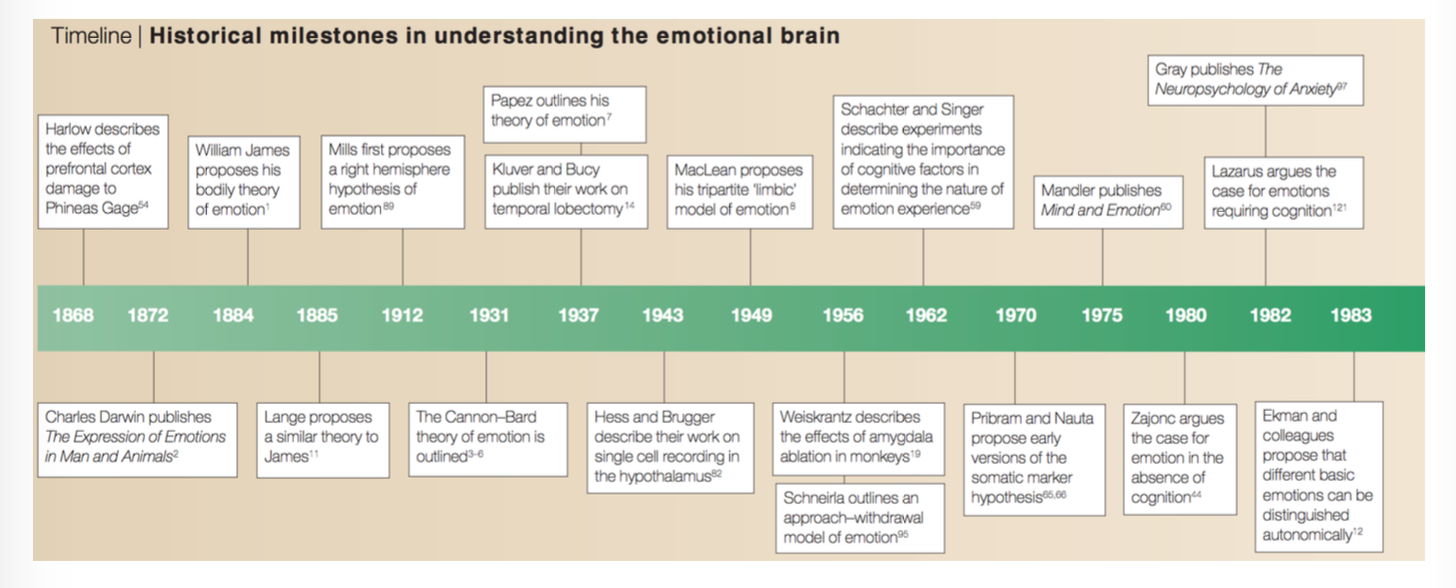
\includegraphics[width=5in]{figure/timeline.png}}
	本节将列举几个广泛使用的情绪模型:
	\begin{itemize}
		\item James Lange理论。这是发表于1884年的一篇论文,并且首次给出了情绪的定义。这个理论认为身体对外部事件产生的生理反应的结果就是情绪,是由生理学派首创的十分著名的理论。
		\item Cannon Bard理论。这个理论否定了上条理论,他们通过试验,发现无论有没有身体的响应,大脑都会产生情绪。因此,他们认为当来自外界的刺激传入到大脑之后,丘脑和大脑皮层就会被激活,从而产生了情绪。这个理论肯定了丘脑的关键作用,但是完全否定了身体和情绪的联系,这是它的不足之处。
		\item Schachter Singer理论。这个理论认为人们会对自己正在经历的情绪而产生相应的生理反应,并且注重外界环境对这种生理反应的解释。举例来说,譬如一个人在奔跑,如果是遇到了危险而逃命,那么这个理论将情绪解释为害怕;而如果是一个人跑向他喜欢的人,那么可以将这个情绪解释为激动。
		\item Opponent Process理论。不同于上述所有,这个理论从对比和对立的角度解释情绪的产生。每个人的基本情绪都有对立的情绪,当某种情绪特别突出,压过了它的对立部分,那么我们就认为自己产生了这个情绪。这个理论十分适合解释吸毒成瘾,吸毒上瘾者为了不断体验到毒品带来的感受,就会不断的吸毒,并且越来越严重。
		\item Papez Maclean理论。 Papez提出了环路理论,解释了整个情绪产生的通路,也就是从外部的刺激到产生情绪信号的大脑内部的整个通路。 Maclean在这个基础上又提出了内脏脑,它的职能是调节与情绪相关的组织和器官,并且通过丘脑调节内脏和骨骼的相应反应。
	\end{itemize}
\section{情绪分类与情绪分类模型}
	一直以来,都有两种不同的观点来进行情绪的度量。一种认为情绪是离散并且是可以相互叠加从而派生出新的情绪的。另一种是认为情绪是连续的并且可以进行测量,他们之间只有强度的差别。本论文的基本观点是情绪可以分成多个类别的。
	\centerline{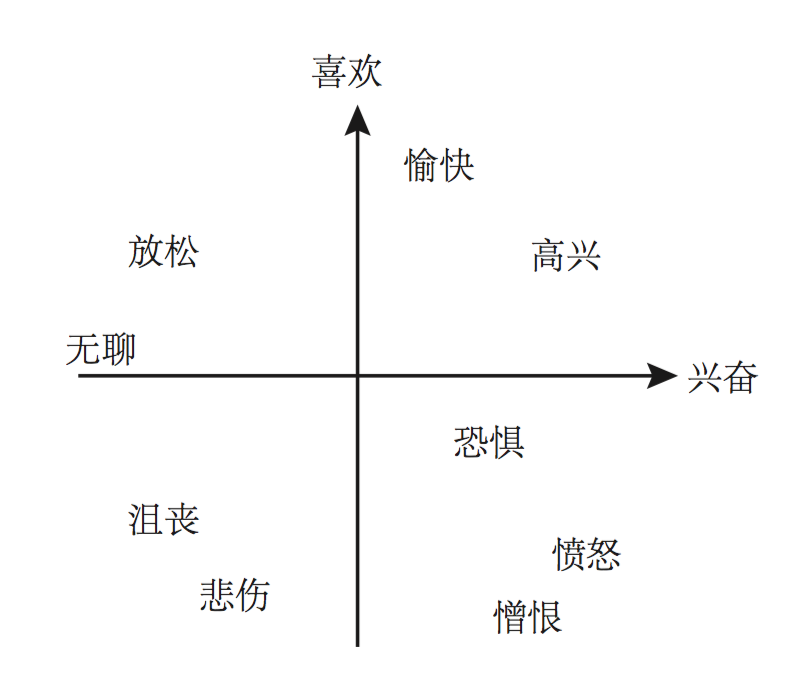
\includegraphics[width=3.5in]{figure/emotion.png}}
	 \subsection{基本情绪}
	 P. Ekman提出的理论认为情绪是离散可叠加并且可以独立的被测量。他最有影响力的研究成果是有六类基本情绪是跨越了种族和国界而广泛适用于人类中的,基于他的研究成果,他提出论点认为人的情绪需要分成六种:愤怒,悲伤,高兴,恐惧,厌恶和惊愕。 而James的情绪集合却包括了愤怒,恐惧,悲伤等\upcite{emotion}。Clynes的情绪集合包括了愤怒,厌恶,悲哀,快乐,浪漫,仇恨,中性等等。Izard的情绪集合包括了愤怒,悲伤,害怕,关心,内疚,快乐等等。
	 
	 不但情绪的划分如此众口不一,我们还很难找到明确的标尺去区别不同的情绪。随着这些年科研工作者的努力,我们才渐渐可以得知不同情绪之间的联系。譬如愤怒的情绪可以转变成为悲伤的情绪。为了让这种关联可视化,我们采用Lange的情绪分类模型,见上图。纵坐标表示的是人们的愉悦度,从厌恶到喜欢。横坐标表示兴奋程度,从低迷到兴奋。这样一来,多种不同的情绪就可以分解开来,通过这个两维度的坐标系显示出来。
	 
	 特别地,J. Panksepp在上世纪提出了大脑中情绪的定义,给出了四种最基本的情绪系统,并且认为这是四种动物出生后不久就拥有的。
	 \begin{itemize}
	 	\item 寻找。 寻找的情绪让情绪的产生者对认识世界充满了好奇,并且进行目的驱动下的寻找,从而找到生存的环境和物品,生存下去。
		\item 害怕。害怕的情绪对疼痛等外界刺激做出反应,害怕情绪的产生会造成战斗,逃遁或者颤栗的行为。
		\item 愤怒。愤怒的情绪通常由于沮丧,外部刺激,身体自由的限制等等引起。
		\item 恐慌。恐慌的情绪通常用于和母亲的分离而引起,它会造成哭泣,叫喊等等行为。
	 \end{itemize}
	 \subsection{多维度情绪表示}
	 利用数据可视化的原理,我们可以在二维模型上将所有情绪描述出来。自然地,相似的情绪状态在二维坐标系中应该距离更近,而相差愈大的情绪状态在坐标系中应该距离更远。通常,心理学家们把这两个用于可视化情绪的维度分别叫做警觉度和效价。后者主要表示情绪的消极/积极程度,而前者代表情绪给人带来刺激的强度。可以用下图(图2-1)表示。
	 \subsection{情绪}
	 虽然在每天平淡的生活中,每个人无时无刻都不被感情充斥着,但是感情却很难完全由自己控制。因此,在实验搜集数据时,我们对能够快速调动并激发实验参与者某些特定情绪和感情的方法有迫切的需求,并且要有较好的可依赖性,鲁棒性和可持续性。在观察了现有研究者尝试过的多种方法以后,论文决定采用视频库作为被试者观看的素材,也就是刺激材料。
	 通过广泛的搜索,本文作者找到了大量汉语作为音频的国内外电影或微电影,排除对英语接受程度不同这个额外变量的影响。不同于P. Ekman提出的六种基本情绪的分类,本文选取高兴,悲伤,中性三种区别最为显著的基本兴趣。在数据收集阶段,实验室通过询问大量与实验参与者各方面条件都类似的学生的评价,根据评价的高低最终选出了15段视频片段作为最终的实验素材。
	 最后,为了保证数据的可信程度和获取足够数量的数据,每个被试都分别进行三次的实验。这也为我们下一步继续研究基于个体的情绪识别研究提供了数据。
\section{本章小结}
	本章对情绪的定义,种类,分类的不同方式和情绪的二维可视化方法做了基本介绍。基于上述的情绪评价模型,本文针对相关需求使用了特定的素材,最终采集到了适合进行EEG和眼动仪信号多模态分析的数据。


%# -*- coding: utf-8-unix -*-
%%==================================================
%% chapter06.tex for SJTU Master Thesis
%%==================================================

%\bibliographystyle{sjtu2}%[此处用于每章都生产参考文献]
\chapter{脑电与情绪相关背景}
\label{chap:chap2x}

\section{大脑结构和对应功能分布}
	脑是人类高级神经系统的主要组成部分,它包括大脑,小脑和脑干。人类大脑主要分成了脑缘系统,大脑皮质,和脑核。
	
	大脑皮质在大脑的表层上。大脑的中间有一道纵向裂痕,将大脑分成左右两个半球,也就是我们所说的大脑半球。大脑皮质肩负着人类的高级情感和神经方面的功能。大脑皮质主要分为左右半球两部分,每个半球又分别包含了额叶,顶叶,枕叶和颞叶。
	
	在相关学术领域,这四个脑区的研究已经较为深入,针对着四个脑区的功能,目前被广泛接受的理论如下:
	\begin{itemize}
		\item 额叶。
		
			负责高级认知功能,譬如学习,语言,决策,运动,情绪等。
		\item 顶叶。
		
			负责躯体感觉功能,视觉功能,空间位置处理功能等。
		\item 颞叶。
			
			负责听觉,嗅觉等功能。另外还负责了长期记忆功能等。
		\item  枕叶。
		
			高级视觉处理的功能。
	\end{itemize}
	
\section{脑电产生原理}
	
	脑电是头皮部位的电位活动。测量脑电,测量的是大脑神经元里面产生的电流和典雅波动。
	
	大脑里的电荷分布在了数亿的神经元中,而神经元之间通过膜转运蛋白对离子的转运来放点。神经元无时无刻不在与外环境进行离子交换,来维持静息电位或者激发动作电位。根据电荷同性相斥异性相吸的原理,当带有相同电荷的离子离开神经元的时候,就会排斥周围环境相同电荷的离子,通过这样一个链不断传递下去,就形成了波,而上述过程就是容积导电。当离子形成的波传播到了头皮和我们的采集电极,电极里的电子就会运动。而这种电子运动会让不同位置上的电极产生电压差,我们可以测量出来这个电压差,并且随着时间记录,这就是脑电图。
	
	一个神经元产生的电压太小,无法被脑电图记录下来,所以我们测量出来的脑电图,往往是非常多空间中邻近的神经元的同步活动。如果神经元不是空间中邻近,那么他们的同步活动很难被记录。皮质椎体神经元排列整齐,并且行为往往一致。所以经常是脑电信号产生的主要神经元。 由于电压随着距离的增加而平方衰减,大脑内部的脑电相对于靠近头骨的脑电更难被记录。
	
\section{采集脑电}

	常用的脑电采集的方法是用胶状脑电膏把电极和头皮粘在一起。这样一来因为头皮到电极的电阻被减小,脑电信号会更容易采集。这种方法虽然能采集到清晰的脑电信号,但是由于脑电膏涂抹的工作十分复杂,并且被试的实验过程将会变得不舒适,现在实验室采用的是干电极直接与头皮接触采集脑电信号,避免了脑电膏的使用。
	
	我们根据国际上被广泛使用的10-20系统来规范电极在头皮上的摆放位置[参考文献,drn32]。这个规范对电极位置的安排十分对称,使得采集到的脑电信号较为完善。 根据这个规范,我们选用了62导电极的采集方法。下图所示是62导电极采集方法的图示。
	
\section{脑电信号频域特征}
	
		不同频带上的脑电信号有不同的生理意义,通常我们将1-50Hz的脑电信号分成了五个频段,分别是Delta, Theta, Alpha, Beta, Gamma。 特征如下所示:
		\begin{itemize}
			\item \textbf{Delta频带}
			
				1-4Hz。Delta频带通常出现在成年人的前额或者婴儿的后脑的位置,并且波幅较大。该频带的脑电往往在成年人睡眠时出现,也可能出现在成年人连续注意的时候。
				
			\item \textbf{Theta频带}
				
				4-8Hz。Theta频带通常出现在幼儿,困倦和刚刚醒来的儿童和成年人中,一般情况下,出现这个频带的脑电信号时,人的意识比较模糊,反应比较迟钝。
				
			\item \textbf{Alpha频带}
			
				8-14Hz。Alpha频带通常被看作是脑电图的基本频带,出现在头的后部或者两边,中间部位较少出现。该频段出现时,对于该频段脑电波在左右脑分布的情况,结果是非主导侧的波幅较大。出现了这个频带的脑电信号时,人们往往在进行休息,反射较为简单。
				
			\item \textbf{Beta频带}
			
				14-31Hz。Beta频带的波幅较小,通常出现在大脑两侧的位置,并且分布对称,前侧的波幅最强。 出现该频带的脑电信号时,人通常处于注意力高度集中的状态,譬如警惕,思考,忙碌等。
				
			\item \textbf{Gamma频带}
			
				31-50Hz。该频带的脑电信号往往出现在负责躯体感觉的皮层,并且往往在人进行多个模态信息的处理中(如嗅觉和听觉,听觉和视觉)出现,同时也常在短时记忆发生的时候出现。
		\end{itemize}
\section{本章小结}

	本章介绍了本文所需要的脑电背景知识,包括在脑电的研究背景。主要介绍了大脑的结构和分区等生理学知识,以及脑电信号采集的原理,脑电产生的生理学远离,并着重介绍了脑电的频域特性。不同区域的差异和不同频段的差异同样是情绪识别研究的热点,而脑电的产生原理和脑电的采集更是实验室的的数据来源,与本文的数据密切相关。
%# -*- coding: utf-8-unix -*-
%%==================================================
%% chapter02.tex for SJTU Master Thesis
%%==================================================

%\bibliographystyle{sjtu2}%[此处用于每章都生产参考文献]
\chapter{数据预处理}
\label{chap:chap3}

\section{脑电信号数据预处理流程}
	在本论文中,在进行多模态深度学习之前,需要先将提取到的脑电原始数据进行预处理,而从原始数据转化到我们的输入数据需要经过三个步骤:消除噪声去除伪迹,特征提取和特征平滑。详细流程图请见下图:\\
	由于脑电十分微弱($\mu$V级),采集EEG信号过程中受到的干扰非常多,因此我们拿到的原始数据并不是纯粹的脑电数据,而在其中夹杂了很多噪音。为了解决这个问题,我们应该首先对原始数据进行合适的预处理,在保留有用的EEG信号的前提下,删除掉夹杂着的噪音信号。另外,由于同一个视频片段的情绪应该是一定的,不会出现突然由令人高兴到令人悲伤的跌宕起伏的情节,所以情绪的变化理应稳定平滑,不应该出现剧烈的改变。因此我们认为EEG信号的剧烈变化是由于非情绪相关的大脑其他活动引起的,譬如回忆。所以,我们同样有必要对数据进行平滑处理,这样就可以消除脑电信号的剧烈抖动,增加信号的稳定性和数据的可信度。
\section{消除噪声和去伪迹}
	由于上述原因,我们总结出了以下几种干扰,都是由非情绪相关的大脑活动产生的。
	\begin{itemize}
	\item 眼电伪迹:大脑发出控制眼球的指令就会产生电流,从而形成这种与情绪无关的脑电信号,对于我们的原始数据而言,它是需要去除的噪声。频率为1-50Hz.
	\item 肌电伪迹:由于人不可能保持完全静止的状态,所以肌肉的运动会产生脑电信号,对比于反应情绪的微弱脑电信号,肌电信号可以达到相当大,产生很大程度的污染,大大影响我们提出的数据。
	\item 心电伪迹:心跳的过程也会产生电场和脑电信号,作为我们数据的噪声,频率大约在1Hz。
	\item 皮电干扰:由于人的排汗和空气湿度变化,涂抹在脑电电极周围的脑电膏会产生一定程度的浓度改变等,影响脑电信号的稳定性,从而产生了噪声。
	\end{itemize}
	
	我们首先对原始数据进行降采样,采样率为200Hz。另外,由于1-50Hz的脑电信号是具有明确生理意义的,所以我们才去原始数据以后先进行滤波,提取出1-75Hz的信号,这一步即可消除大部分噪声。

\section{脑电特征提取}
	原始数据经过降采样之后依旧是在时域上,为了保持与之前实验室成果的对比,以及利用EEG信号在频域上的生理意义,本论文采用EEG的频域特征作为输入特征,并分析其与情绪的关系。
	\subsection{时域到频域的特征变换}
		在这个步骤中,离散短时傅立叶变换(Short-Term Fourier Transform, 简称为STFT)是常用并且快速有效的方法。
		
		如果我们设$x[n] = {x_1,…, x_n}$为某一电极上,每个时间窗采集到的原始数据样本数。那么我们就可以利用STFT算法得到下式:
		\begin{align}
		STFT{X[n]}(m, \omega_{k}) \heartsuit X(m, \omega_{k}) = \sum_{n = 1}^N x[n]w[n-m]e^{-j\omega_k n}
		\end{align}
		
	其中,k为整数,并且定义区间是[0,N), $\omega_k = \frac{2\pi k}{N}$,并且w是一个窗口函数,它的作用是对每一个窗口独立地进行傅立叶变换,当我们把整个信号按照时序分成很多片段然后每个片段分别进行傅立叶变换,那么就得到了每个窗口所代表时间的频域信号。这样既得到了频域信息,又没有在整个时域直接进行变换,从而保留了部分时序性,减少了原始信号的时间方面的信息丢失,也为之后对循环神经网络等需要时间信息输入的研究提供了数据。
	
	汉宁窗是常见的窗口函数,也是本论文所使用的。定义如下:
	\begin{align}
	 w[n]=\left\{
	\begin{aligned}
	x & = 0.5[1-\cos(\frac{2\pi n}{M - 1})] ,  & 1 \leq n < M\\
	0 &, & otherwise \\
	\end{aligned}
	\right.
	\end{align}
	
	经过多次试验和测试,我们决定采用窗口大小为4秒的汉宁窗函数。
	
	现在的研究有充分的证据证明,1-50Hz频段的脑电信号有明确生理意义,它被更细的划分为代表1-4Hz的Delta频段, 4-8Hz的Theta频段,8-13Hz的Alpha频段,13-30Hz的beta频段和30-50Hz的Gamma频段。我们首先利用傅立叶变换得到每个频段的信号,然后再利用傅立叶变换计算的到每个频段的能谱:
	\begin{align}
	E(\omega_k) = X(m, \omega_k) * X^*(m, \omega_k)
	\end{align}
	其中*代表的是共轭函数的意思。
	
	经过傅立叶变换和后续计算以后,我们得到的EEG信号有62个频道,而每个频道可以分成5个更细的频段,所以我们最终的特征就是310维的向量,也就是我们深度学习网络的输入向量。
	\subsection{微分熵特征}
	微分熵(英文Differential Entropy,简称DE)由香农熵拓展而来,它描述随机变量的熵。
	设随机变量X,则X的概率密度函数$p(x)$的支持为集合C.那么它的微分熵$h(X)$可以由下式表示:
	\begin{align}
	h(X) = -\int_C f(x)logf(x)dx
	\end{align}
	自然地,我们可以用高斯分布来作为脑电信号的分布的假设,如此便可获得脑电信号离散序列的微分熵如下:
	\begin{align}
	h(X) &=  -\int_{\infty}^{-\infty} {\frac{1}{\sqrt{2\pi \sigma^2}} e^{\frac{{(x-\mu)}^2}{2\sigma^2}}log(\frac{1}{\sqrt{2\pi \sigma^2}}e^{\frac{{(x-\mu)}^2}{2\sigma^2}})dx} \\
	&=\frac{log(2\pi e \sigma^2)}{2}
	\end{align}
	通过对式(3-6)的分析,我们可以看出EEG信号的DE特征只与$\sigma^2$有关,同时,在去除了平均值以后,我们可以通过下式得出EEG信号的方差:
	\begin{align}
	\sigma^2 = \frac{1}{N} \sum_{i=1}^{N}{{x_i}^2}
	\end{align}
	根据式(3-7)我们可以看出方差$\sigma^2$与能量$P_i$是正比关系,因此再根据式(3-6)可得下式:
	\begin{align}
	h_i(X) = \frac{1}{2}log(2\pi e \sigma_i^2) = \frac{1}{2}log P_i + \frac{1}{2}log(\frac{2\pi e}{N})
	\end{align}
	经过进一步简化,我们可以得到下式:\\
	\begin{align}
	h_i(X) = log P_i
	\end{align}
	
%# -*- coding: utf-8-unix -*-
%%==================================================
%% chapter04.tex for SJTU Master Thesis
%%==================================================

%\bibliographystyle{sjtu2}%[此处用于每章都生产参考文献]
\chapter{设计情绪实验}
\label{chap:chap4}

\section{收集情绪刺激视频}
	由于需要采集人的情绪,所以进行实验的第一步是收集视频作为诱发被试情绪的材料。实验室所选择实验材料的标准如下:
	\begin{enumerate}
	\item 为了避免由于对英语熟悉程度不同而造成的理解差异,我们仅选择汉语配音的视频。
	\item 由于本实验被试几乎全部是在校本科生和研究生,所以实验材料尽量选取符合大学生价值取向,容易被大学生理解并激发其相应情绪的。
	
	\item 影片符合基本当代价值取向,不包含极端内容和思想。
	\item 每个片段长度尽量选取在1-4分钟,既可以采取到相应情绪的数据,也保证不会有很多冗余内容造成了中性(无聊)的情绪。
	\end{enumerate}
	
\section{情绪刺激视频筛选}
	由于采取到的负荷上述要求的视频片段的数量非常多,如果采用全部片段作为实验素材,那么实验的耗时会太长。因此,需要筛选出最合适的素材。为了解决这个问题,实验室采用Alexander S.所提出的标准来评价收集到的素材,并根据来自志愿者的评价来对这些素材进行评估。
	志愿者需要填写的问卷表对每个影片素材都有二十多项标准,包含了譬如激发程度,感兴趣程度,热情程度,哦那个剧程度,失落程度,警惕程度等等。每一项都从1-5中选一数字进行打分,数字越大则代表感受到的响应程度越深。最后,我们对这些问卷就行统计和评估,选出了最适合的十五段情绪。去除了容易令人迷惑的片段,最终结果和目的则是增加了实验数据的可信度。
	
\section{情绪刺激实验流程}
	本论文中采用ESI Neuroscan平台进行EEG信号的采集和记录。在被试戴好脑电帽,所有电极都测试妥当之后,他会进入实验室的真车环境中观看大屏幕。每个被试进行三次实验,每次实验中均为15个视频片段。除此之外,每个片段开头会有剧情简介,让被试有心理准备,获得更好的情绪激发效果。
\section{本章小结}
	本章主要介绍了实验素材的收集,筛选和实验的基本流程。
%# -*- coding: utf-8-unix -*-
%%==================================================
%% chapter06.tex for SJTU Master Thesis
%%==================================================

%\bibliographystyle{sjtu2}%[此处用于每章都生产参考文献]
\chapter{多模态深度学习算法}
\label{chap:chap6}

\section{深度学习介绍}
	深度学习是最近开始吸引到越来越多研究者注意的一类基于深度神经网络的机器学习算法。深度学习的模型的 一个共同特点是它们都是由感知器构成的多层神经网络,且层数一般较多(通常三层)。 深度学习通过组合更加具体的底层特征,形成了更加抽象的高层表示,从而发现输入数据的高层的特征表达。
	
	深度学习出现之前,学者们普遍使用反向传播算法训练层数较多的神经网络,但这种方法存在着诸多弊端。
	\begin{itemize}
		\item 梯度消失问题,随着层数的增加,梯度在反向传播的过程中逐渐 变成接近于 0 的很小的数,导致权重更新缓慢,训练效率低下;
		\item 由于参数过多,容 易导致过拟合问题。
	\end{itemize}
	
	这些问题一直阻碍者神经网络层数的增加,因而学者们无法抽象得到更高层次的特征。然而,Hinton提出的逐层的无监督训练深度新年网络的方法带来了希望,也越来越受到机器学习研究者的青睐。随口,深度学习在图像识别和文本分类等任务中都表现出了卓越的性能,令人满意 下面介绍深度学习的常用模型。
\subsection{深度自编码器}{
	本论文所使用的算法模型是基于深度自编码器的,具体的实现将在下一节中详细说明。本节目的是阐述深度自编码器的原理。
	
	根据定义,深度自编码器是由两个对称的深度置信网络组合而成。一般情况下,会有四到六层的编码层,紧跟着的是同样层数的解码层,并且编码和解码对应的每层结构都完全相同。每一层都可以认为是受限波尔兹曼机(Restricted Boltzmann Machines,简称为RBM)\upcite{Fischer:2014:TRB:2533326.2533561}。编码层和解码层交汇之处就是深度自编码器学习到的的特征向量。
	
	
	在编码阶段,举例来说,譬如我们的输入数据是310维的,那么通常来讲,深度自编码器的第一层应该有略多于输入层元素个数的维度,譬如350维,这看上去有些让人困惑,因为我们都知道创建比输入维度更多的参数容易造成过拟合。但是实际上,拓展出更多的参数就相当于表示了更多输入数据的特征,只有这样才能实现最终的解码过程,这是由于sigmoid函数的表达能力决定的。一旦sigmoid函数进入饱和区,那么就会丢失很多信息,让深度自编码器的第一层有更多参数是为了补偿sigmoid函数这方面的不足。而在第一层之后,在编码的阶段里,维度应该逐层指数递减,直到最后一层,此时不进行任何分类,而只是一个RBM的隐层。我们建立好编码网络,然后在后面加上解码网络。
	
	在解码阶段,输入就是编码阶段的最后一层,这一层也就代表了编码之后的信息。正如前面所说,解码网络与编码网络对称,它的训练过程就是学习如何用编码之后的信息来重建原始输入。初始化的时候并不能随机初始化,而我们应该设置所有参数等同于编码网络对应的部分(连接权矩阵需要转置)。整个网络是利用反向传播算法来进行训练的,每次对比解码网络重建出来的值和原始输入的差,利用损失函数来计算梯度,最后更新。
	
	在利用反向传播算法进行训练的阶段,学习率应该设置的很小,有建议说对于二进制数据,学习率应该设为$1 * 10^{-3}$,而对于连续数据,学习率应该设为$1 * 10^{-6}$。
	
	深度自编码器已经在多个领域有实际应用。
	\begin{itemize}
	\item 图像搜索,可以将较大的二维图像特征向量,譬如上千维的像素编码成到长度为几十的特征向量。加速搜索,返回准确结果。
	\item 数据压缩,如语意哈希(Semantic Hashing)\upcite{Salakhutdinov09semantichashing}。这是一种为文件寻找一种二进制编码的方法,使得相似度高的文件对应的编码海明(hamming)距离小,相似度低的文件对应的编码海明(hamming)距离大。可以加速文件搜索等。
	\item 主题模型和信息检索\upcite{Blei:2003:LDA:944919.944937}。深度自编码器可以用于自然语言处理里面的主题模型或者类似的利用统计学来在一系列文档里面建立主题的算法。具体来讲,每个文档都被转化为bag-of-word模型,也就是词频统计的特征向量,然后把词频归一化,所以每个元素都可以被认为是一个词在文档中出现的频率。接着把这个特征向量输入进由多层RBM组成的深度置信网络,并且设定网络的最后一层只有比较少的元素,譬如10个。最后,把这一层的特征作为新的特征向量,每个特征向量与一篇文档一一对应。这样每个文档可以与任何一个其他文档计算距离,距离由新的特征向量所定义。相似的文档距离近,如此一来,特征向量相似的文档应该具有类似的主题。这就是主题模型的工作原理。
	\end{itemize}
}
\subsection{深度信念网络(Deep Belief Networks), DBN}{
	  深度信念网络\upcite{NIPS2007_3363}是一个生成的概率模型,与传统的神经网络的判别模型相对,生成的模型是建立一个观察到的数据和标签(label)之间的联合分布,对$P(Observation|Label)$和 $P(Label|Observation)$都做出了估计,而判别模型只需要评估后者,\\ 也就是$P(Label|Observation)$。自然的,研究者一开始对于深度信念网络也使用了传统的反向传播算法,对于在深度神经网络应用传统的反向传播算法的时候,深度信念网络遇到了很多问题,譬如:
	  \begin{itemize}
	  	\item 训练集合需要有标签,否则无法进行反向传播算法来学习整个网络。
		\item 因为网络很深,迭代一次需要计算非常多层数的参数,包括求梯度,所以过程比较缓慢。
		\item 若参数不够合适,那么最终结果很可能收敛于一个局部最优解,而不是全局最优的。
	  \end{itemize} 
	  
	  深度信念网络是多个受限波尔兹曼机不断叠加而成的,一个深度信念网络的连接就是通过自顶向下的生成权值来指导,从而确定的,受限波尔兹曼机就像一个个砖头一样,构建出了深度信念网络这一面墙,相比传统和深度分层的sigmoid信念网络,也就是传统的神经网络,它能易于连接权值的学习,可以达到更好的结果,训练的速度也会加快,还可以避免很多发散的情况。而这个优化的关键之处就在于对每个受限波尔兹曼机进行非监督贪婪逐层的方法来预训练,从而获得生成模型的权值,而不是随机初始化。受限波尔兹曼机的训练和学习过程将会在下文被详细阐述。 
	  
	  利用这种方法,训练时间会显著的减少,因为只需要单个步骤甚至就可以接近极大似然学习。添加进入网络的每一层都会改进训练数据的对数的概率,我们可以理解为越来越接近数据集能量的真实表达。这个拓展意义重大,无标签数据的利用同样如此,他们都是任何一个深度学习应用的决定性的因素。
	  
	   在预训练结束后,深度信念网络可以利用带标签数据用反向传播算法去对判别,从而对做调整,有更好的性能。在这里,一个标签集将被附加到顶层,来推广联想记忆,具体是通过一个自下向上的,学习到的权值获得一个网络的分类器。这样训练的性能会比单纯的反向传播算法训练的网络好。我们可以很直观的解释,深度信念网络的反向传播算法只需要对权值参数空间进行一个局部的搜索,而不是像前向神经网络一样要从头到尾进行全局搜索,所以这相比前向神经网络来说,训练是要更快的,而且进行到收敛,需要的时间也更少。
	   
	   非常值得注意的是,虽然深度信念网络和深度堆叠波尔兹曼机看起来非常相似,但两者差别却是十分巨大。最重要的一点本质区别就是深度信念网络是有向图,而深度堆叠波尔兹曼机是无向图。我们可以把深度信念网络认为是有很多层数和参数,并且紧密相连的sigmoid函数的信念网络。而可以把深度堆叠波尔兹曼机看作是有很多层数和参数,并且紧密相连的马尔科夫随机场。
}
\subsection{卷积神经网络(Convolutional Neural Network, CNN)}{
	\centerline{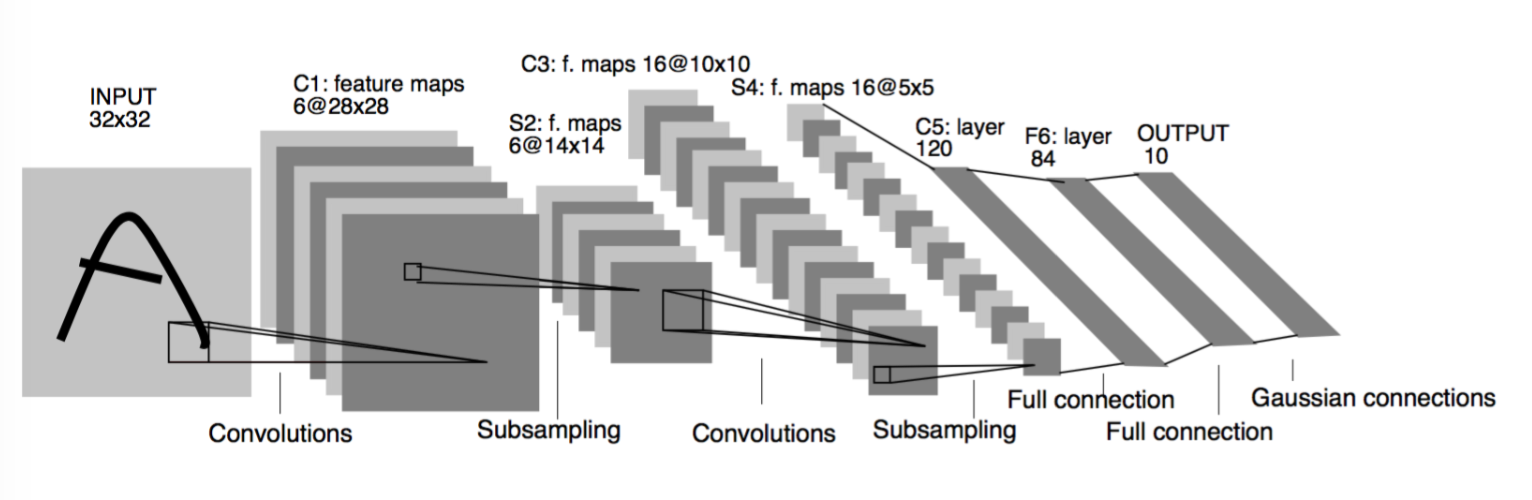
\includegraphics[width=5in]{figure/cnn.png}}
	卷积神经网络是专门为了针对解决图像处理问题而提出的算法模型,针对图像的二维特征,卷积神经网络可以直接以二维图像作为输 入。卷积神经网络包含卷积层和降采样层两种不同的单层。卷积层通过不同的核函数进行卷积 的运算,对图像进行特征提取。一般而言,解决图像的问题,研究者需要多个核函数,提取出图像中不同 的特征,然后把这些特征组合起来一起学习。
	
	卷积层将原始的图像处理成很多张不同的特征映射图,降 采样层的目的是为了减少参数,避免大量的运算和过拟合。经过多次卷积层和降采样层后,原始图像可以被抽象表示为高层次的特 征,也就寻找到了更有代表性的特征,可以帮助我们进行图像识别等任务。卷积神经网络的典 型结构如上图所示。常用的卷积神经网络模型有 LeNet \upcite{Lecun98gradient-basedlearning},  ZFNet \upcite{DBLP:conf/eccv/ZeilerF14}, GoogLeNet \upcite{Szegedy_2015_CVPR}, VGGNet \upcite{DBLP:journals/corr/SimonyanZ14a}和 ResNet \upcite{DBLP:journals/corr/HeZRS15}。
	
	具体的,卷积神经网络利用局部感知和参数共享两种优化方法,大大减少了计算复杂度。
	\begin{itemize}
		\item 局部感知。按照定义,卷积层应该对图像拥有全部的视野,每个像素都应该与卷积层的每个元素有边相连,因此产生了巨大数目的连接权。局部感知这种优化方法就是给每个卷积层的元素限定视野,让每个卷积层的元素只与图像的部分像素相连,这样一来,卷积层的所有元素刚好覆盖整个图像,可以让网络的参数减少多个数量级,让训练变的可能。
		\item 参数共享。即使使用了局部感知的方法,每个卷积层的元素还是各自拥有多个参数,随着卷积层的元素的数目变大,计算复杂度仍旧非常高。参数共享的意义在于把卷积层的每一个元素的对应权值都设为同一个,也就是让所有卷积层的神经元共享参数。这个方法可以再次让网络的参数减少多个数量级。并且可以很直观的理解:卷机操作可以看成是特征提取的方式,而这个特征提取与位置无关。这其中隐含的原理则是:图像所有部分的统计特性都相同。这就意味着,同一幅图像在一部分学习的特征还能用在另一部分上,所以对于这个图像上的任意区域,我们都能使用同样的学习特征。
	\end{itemize}
	这两个优化方法使得卷积神经网络在图像处理领域的表现十分优秀,深受研究者的青睐。
}

\subsection{递归神经网络(Recurrent Neural Network, RNN)}{
	\centerline{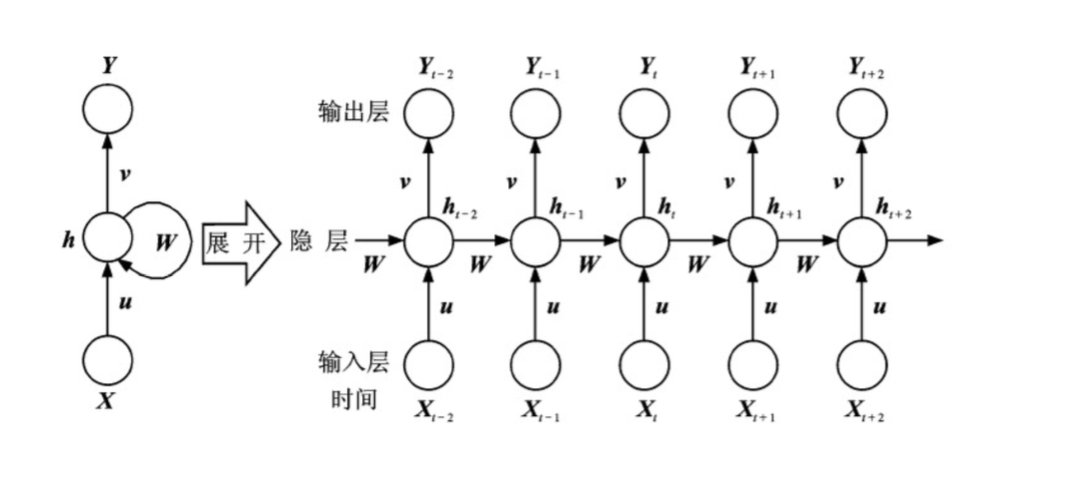
\includegraphics[width=4.5in]{figure/rnn.png}}
	递归神经网络\upcite{Schuster:1997:BRN:2198065.2205129}的目的使用来处理序列数据。在传统的神经网络模型中,是从输入层传递到隐含层再传递到输出层,相邻的两层之间是全连接的,每层之间的节点是没有任何连接的。但是这种普通的神经网络对于很多问题却表现的不够好,甚至无能为力。譬如,你要预测句子的下一个单词是什么,一般需要用到前面的单词,因为一个句子中前后单词并不是独立的,而是跟上下文有关。它之所以称为循环神经网路,本质就是一个序列当前的输出与之前时间的的输出也有关。具体的表现形式为网络会对之前时间的的信息进行记忆并应用于当前时间输出的计算中,即隐藏层之间的节点不再是没有任何连接,而是有连接的,并且隐藏层的输入不但包括输入层的输出,还包括上一时刻隐藏层的输出,隐藏层跟隐藏层之间额外的相连是递归神经网络的特点。
	递归神经网络是一种具有反馈的神经网络,其输出不但与当前输入和网络的权值有关,而且还与上一个时间点网络的输入 有关。递归神经网络通过添加跨越时间点的隐藏层,把时间因素考虑在内。也就是说,隐藏层 的反馈,不仅仅进入输出端,而且还进入了下一时间的隐藏层。递归神经网络的结构如上图。
	
	因为一旦展开,它可以有非常多层,所以递归神经网络被认为是最深的神经网络。递归神经网络结构上具有天然事件序列联系的特点,使得递归神经网络能够更好地学习到序列数据的信息和其中分布,即递归神经网络能够自然的考虑输入数据时序上的关系。这在自然语言处理和语音信号处理等时序信号的处理领域有卓越的性能。类似的,正因为脑电信号也是时序信号,并且我们认为人的情绪不是突然改变的,而是缓慢变化的,考虑脑电信号的时序特性是很自然的。}

\subsection{长短时记忆网络(Long Short-Term Memory, LSTM)}{
	\centerline{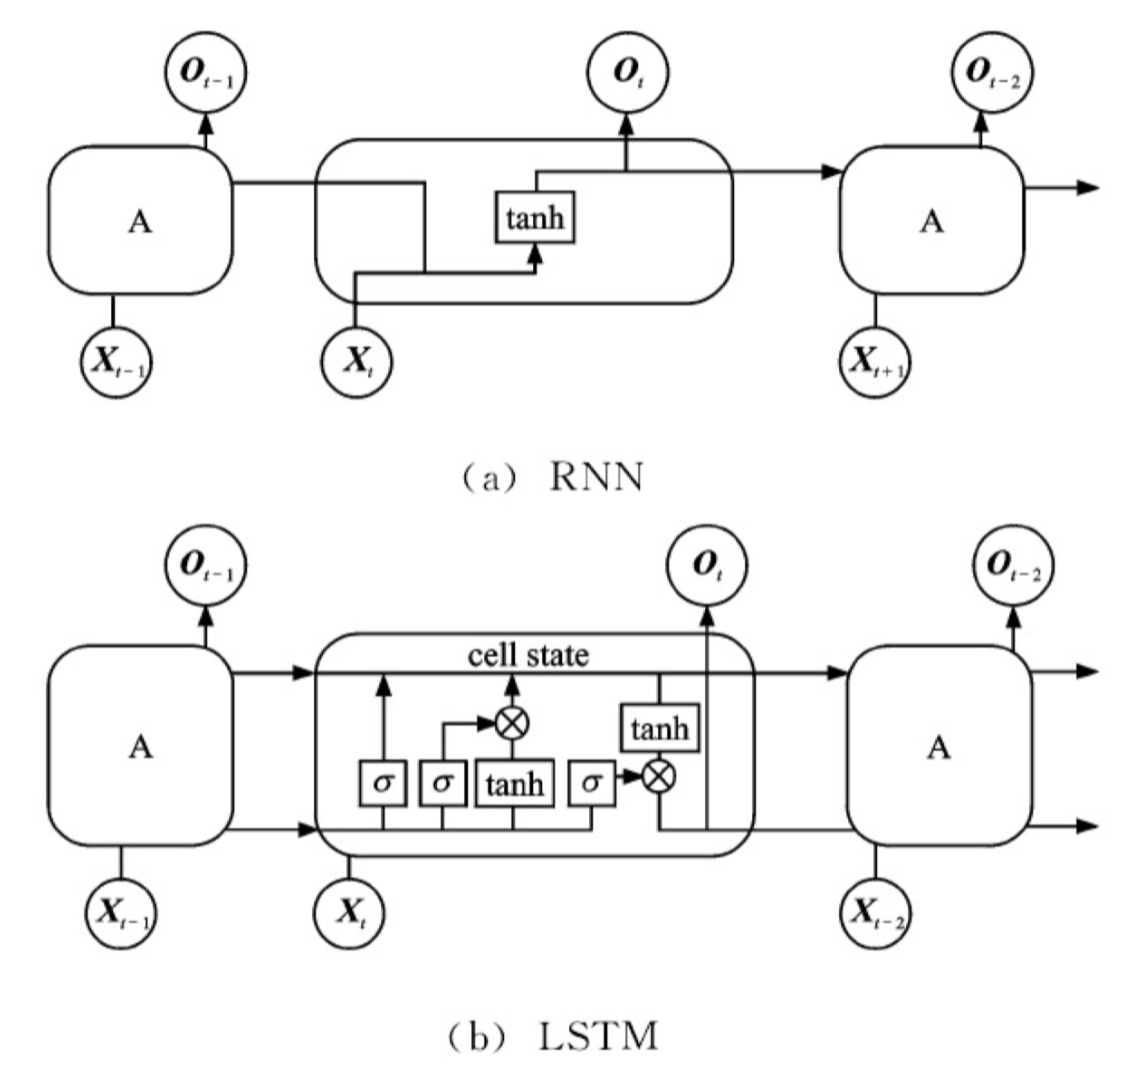
\includegraphics[width=4.5in]{figure/lstm.png}}
	长短时记忆网络\upcite{Hochreiter:1997:LSM:1246443.1246450}是一种特殊的递归神经网络模型, 它是为了解决递归神经网络模型梯度消失的问题而提出的。在传统的递归神经网络中,训 练递归神经网络也是在传统的反向传播算法基础上加上对时间的考量,我们称这种方法位反向时间传播 BPTT(Back Propogation Through Time)。即从上层获取残差而改变本层的内部参数和权值,这些内部参数和权值可以用于计算表示。但是当传播时间比较长,网络比较深的时候,传回的残差会 指数下降,因为每一层都可能会缩小一个数量级以上,这导致网络权重更新缓慢,递归神经网络的长期记忆功能就无法体现。往往此时递归神经网络就可能变得非常难以训练,梯度信号会变得极其微小,近乎为零,或者干脆不收敛,这就导 致递归神经网络梯度消失或者梯度爆炸的问题。因此需要一个存储单元来帮助实现递归神经网络的长期记忆,长短时记忆网络模型由此被提出。
	
	长短时记忆网络的网络结构如上图所示。从图中可以看出,递归神经网络和长短时记忆网络最大的区别在于: 长短时记忆网络中最顶层多了一条名为细胞状态的信息线,也就是这里在存储记忆信息。长短时记忆网络的核心元素是细胞状态,也就是上图中,长短时记忆网络原理图最顶层的传送呆。细胞状态可以被看做传送带,其实就是整个长短时记忆网络模型中的记忆空间,跟随时间而改变。自然的,传送带本身是无法控制哪些信息被记忆,哪些不被记忆,而是控制门决定了哪些信息将被记忆。
	
	长短时记忆网络通过控制门的结构来改变细胞状态的信息。控制门可以让信息有选择的通过。控制门的结构是由一个 sigmoid 函数和点乘操作来组成;sigmoid 函数值的区间为 [0,1] ,点乘操作可以决定信息通过的数量,当结果为0的时候,没有任何信息被传送;当结果为1的时候, 信息全部被传送。长短时记忆网络中有 3 个控制门,分别是输入门,输出门和记忆门。记忆门用来选择删除,也就是忘记过去的某些信息,输入门用来记忆当前的某些信息,经过输入门和记忆门,将过去 和现在的信息和记忆进行合并,并在输出门输出最后的信息。
}

	然而随着图像和文本这两个模态的信息伴随彼此而一起出现的情况与日俱增(譬如微博的图片和文本),如何利用图像和文本之间的匹配关系,挖掘出他们的共有信息成为了多模态深度学习的目标。部分已有研究(需要加注释,引用)对图像和文本的多模态深度学习已经有了比单一模态的深度学习显著优秀的结果。因此,本课题就是在利用多模态的信息来进一步提升情绪识别的效果。本文利用EEG数据和眼动仪数据作为两个模态的输入,尝试寻找两者的匹配关系,并构建共有特征表达,虽然EEG数据和眼动仪数据两者不但在量级还是特征维度上的差别都十分巨大,但是我们仍旧达到比单一使用任意一个模态进行深度学习更好的效果。

\section{算法模型}
	我们的目的是设计合适的网络能够接受两个模态的输入,而输出两个模态的共有特征。自然的,我们选用深度神经网络(Deep Neural Network,简称DNN)作为基本框架。不过传统的DNN都是针对单模态的,于是,我们构建了以RBM为基本单位的,多层次的多模态DNN。它可以接受两个模态的输入,并进行编码和解码过程,最终解码过后可以得到重建后的两个模态的特征。此时我们对重建后的特征和输入特征进行对比并且校正,多次迭代DNN网络就可以得到合适的网络参数,并且可以提取出网络中任意层次的共有特征表达。
	\subsection{RBM介绍}
	如果要进行深度学习的研究,那么必须要理解RBM的相关背景。\\
	\par
	\centerline{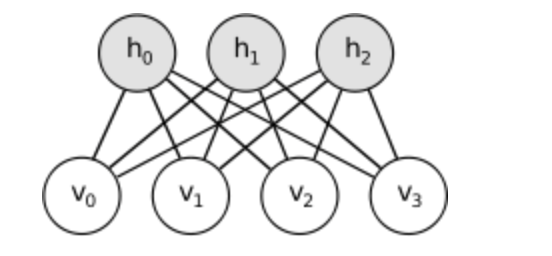
\includegraphics[width=2.5in]{figure/rbm.png}} %要居中就用centerline,这里的图片和tex 文件在一个目录下
	\centerline{图6-1 RBM模型}

	这是RBM的基本模型,其中v代表显层, h代表隐层。每个RBM都由一个显层和一个隐层组成,显层和隐层都可以有大于等于一的任意多个维度。而显层之间的所有单元均不相连,隐层之间的所有单元也全不相连。而两层之间的单元全相连。值得一提的是,如果所有单元保持全相连,那么这个模型就是波尔兹曼机(Boltzmann Machine),由于计算复杂度等原因,深度学习研究者通常使用RBM来构建深度网络。
	RBM是一个基于能量的模型(Energy-Based model),众所周知,一个基于能量的概率模型的概率分布由它独有的能量函数定义。对于常用的伯努利RBM来说,它的能量函数如下:
	\begin{equation}
	\begin{cases}
	E(s) = -\sum\limits_{i=1}^{n-1}\sum\limits_{j = i + 1}^{n} w_{ij}s_is_j - \sum\limits_{i=1}^n \theta_i s_i \\
	p(x) = \frac{e^{-E(x)}}{\sum\limits_t e^{-E(t)}}
	\end{cases}
	\end{equation}
	其中$s \in \{0, 1\}^n$  为n个单元的状态向量。 $w_{i, j}$ 为显层第i个和隐层第j个单元之间的连接权,$\theta_i$为第i个单元的阈值。
	若网络中的神经元以任意不依赖输入值的顺序来更新,那么最终达到boltzmann分布,则训练完毕。
	具体更新过程如下:
	\begin{equation}
	\begin{cases}
	P(v|h) = \prod\limits_{i=1}^d P(v_i |h)\\
	P(h|v) = \prod\limits_{j=1}^q P(h_j |v)\\
	\end{cases}
	\end{equation}
	
	\begin{align}
	\Delta w = \eta(vh^T - v\prime {h\prime}^T)
	\end{align}
	然而由于伯努利RBM只允许显层和隐层的阈值在0,1之间,并且进行抽样更新的过程只能是1或者0。而我们的数据是在实数集上,虽然我们可以对数据进行针对每一维的归一化,从而让伯努利RBM变得可行,但是经过多次试验,我发现不同的归一化方法会产生各不相同的最终结果。为了解决这个这个问题,高斯RBM是一个不错的解决方法。它与伯努利RBM的区别在于更新过程和能量函数的计算。以下是它的具体计算方法:
	\begin{equation}
	E(v,h | \theta) = \sum\limits_{i=1}^{n_v}\frac{(v_i - b_i)^2}{2\sigma_i^2} - \sum\limits_{i=1}^{n_v}\sum\limits_{j=1}^{n_h} W_{i,j}h_j\frac{v_i}{\sigma_i} - \sum\limits_{j=1}^{n_h}c_jh_j
	\end{equation}
	
	\begin{equation}
	\begin{cases}
	P(v_i = v|h) = \mathcal{N}(v | b_i + \sum\limits_{j}h_jW_{ij}, \sigma^2)\\
	P(h_j = 1|v) = sigmoid(c_j + \sum\limits_i W_{ij} \frac{v_i}{\sigma_i^2})
	\end{cases}
	\end{equation}
	
	在根据隐层更新显层的过程中,需要根据b(显层阈值)和$\sigma_i$来确定这个神经元的高斯分布,再进行抽样。根据均值和标准差确定分布,获得抽样。
	
	在根据显层更新隐层的过程中,根据c(隐层阈值) 来确定伯努利分布,再进行抽样。 均值也就是$p(h_j| V)$, 根据这个值来确定分布,进行抽样。
	
	RBM的训练过程就是多次抽样和更新的过程。这也是一个马尔科夫链(Markov Chain)收敛的过程,每一步都是吉布斯采样(Gibbs Sampling)。吉布斯采样是用来构造多变量概率分布的随机样本的方法,特别常用于期望很难计算出来,而条件概率比较容易的得到的情况。
	
	N个元素的联合分布的吉布斯采样过程如下:每次分别对于一个元素采样,总共采样N次,就得到一个样本。具体算法如下:
	
	initialize $x_i$ : i = 1, 2, …, n, T samples:
	
	for t in range(1, T):
	\begin{flalign}
		\qquad \qquad &x_1^{(t+1)} \sim p(x_1 | x_2^t, x_3^t,…, x_n^t)&\\
		&x_2^{(t+1)} \sim p(x_2 | x_1^({t+1)}, x_3^t,…, x_n^t)&\\
		&……&\\
		&x_j^{(t+1)} \sim p(x_j | x_1^{(t+1)},…,x_{(j-1)}^{(t+1)},x_{(j+1)}^t,…, x_n^t)&\\
		&……&\\
		&x_n^{(t+1)} \sim p(x_n | x_1^{t+1}, x_2^{t+1},…, x_{(n-1)}^{t+1})&
	\end{flalign}
	
	利用高斯RBM我们取得了比伯努利RBM更好的结果。
		
	然而,如果真的使用吉布斯采样的方法来训练RBM,那么整个过程需要迭代多次,变的十分缓慢。于是,这里本文应用的是对比散度(Contrasive Divergence, 简称CD)算法,它可以大大缩减整个抽样迭代的步数。
	
	CD算法由G. Hinton提出\upcite{hinton06},用于求极大似然问题(Maximum-Likelihood)的近似解。它的基本思想是,我们想要得到P(v)分布的样本,而我们已有了训练样本,可以假设训练样本自然就是服从分布P(v)的。因此,我们的上述算法第一步初始化过程就不再是随机初始化,而是从任意一个训练样本开始。
	
	因此,CD算法的具体步骤是:从样本集合也就是训练集合任意一个样本$v^0$开始,经过k次吉布斯采样。即对于第t步采样,具体算法如下:
	\begin{flalign}
	\qquad \qquad \qquad \qquad \qquad &h^{t-1} \sim P(h|v^{t-1})&\\
	&v^t \sim P(v|h^{t-1})&
	\end{flalign}
	不断迭代我们就得到了样本$v^k$。有了采样出来的$v^k$,我们把它认为是近似的期望,所以就可以计算出梯度的近似值,并且根据其进行RBM的更新了。
	值得注意的是,在实际应用中,往往t等于1,也就是只采样一次就够了,这也就是为什么CD算法会远远快于吉布斯采样算法。
	CD算法的伪代码请见算法6-1。\\ \\
	\textbf{算法6-1}\\
	输入:k(步数), S(训练集合),W(权值矩阵), a(可见层单元阈值), b(隐层单元阈值)\\
	输出:$\Delta W, \Delta a, \Delta b$\\
	第一步:初始化三个输出参数均为0.\\
	第二步:For All v $\in$ S DO:
	
		\qquad $v^0 := v;$
		
		\qquad For t in range (1, k) DO:
		
			\qquad \qquad $h^t= sampleHiddenGivenVisual (v^t, W, a, b)$
			
			\qquad \qquad $v^{t+1}= sampleVisualGivenHidden(h_t, W, a, b)$
			
		\qquad For i in range(1, $n_h$):
		
		\qquad \qquad For j in range(1, $n_v$):
		
		\qquad \qquad $\Delta W_{i, j} += [P(h_i = 1|v^0)v_j^0 - P(h_i = 1|v^k)v_j^k]$
		
		\qquad \qquad $\Delta a_j += [v_j^0 - v_j^k]$
		
		\qquad \qquad $\Delta b_i += [P(h_i = 1| v^0) - P(h_i = 1|v^k)]$
		
	而有了CD算法以后,我们就可以顺利总结出深度网络的基本单元RBM的整个算法了,这是整个深度网络的基础,请见算法6-2。\\ \\ \\ \\ 
	\textbf{算法6-2 RBM训练算法}\\
	第一步:初始化(initialization)
	
		\qquad 给定训练集合S。q
		
		\qquad 给定训练周期J,学习速率l,以及CD-k算法的参数k。
		
		\qquad 给定隐层的单元数目$n_h$,因为可见层单元数目由特征维数决定。
		
		\qquad 初始化a, b, W。三个参数矩阵或向量。\\
	第二步:训练
		
		\qquad For iter in range(1, j) DO
		
		\qquad \qquad 调用CD-k算法,生成$\Delta W, \Delta a, \Delta b$
		
		\qquad \qquad 按照算法6-1来更新这三个参数直到循环结束
		
	\subsection{模型I}
		\centerline{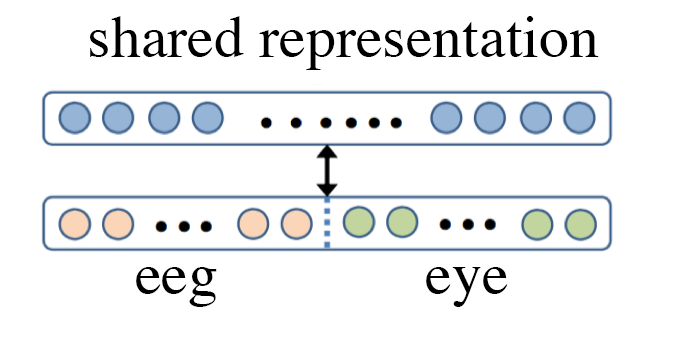
\includegraphics[width=4in]{figure/model1.png}} 
		\centerline{图6-2 算法模型I}
	
	如图所示,这个算法模型的功能是接受两个模态的输入,提取出两个模态的共同特征表达并输出。它的输出可以放到其他分类器,譬如SVM,神经网络等。这是一种比较直观,简单易懂的方法。那就是首先把眼动仪数据(图中eye)和脑电数据(图中eeg)直接进行拼接。设眼动仪数据每个样本有n维,而脑电数据每个样本有m维,那么此时把它们拼接,得到(m + n)维的向量作为每个样本的特征。然后利用预训练之后的RBM进行特征提取,就得到了脑电数据和眼动仪数据的共同特征表达。
	
	然而,这个模型的缺点十分明显,就是这并不是一个深度的学习器,而是一个只有一层的网络,隐层和显层是线性连接的,所以这个模型很难找到眼动仪数据和脑电数据的非线性关系,并不能提取出理想的共同特征。
	
	为了解决这个问题,只能构建更深层次的网络。	
	\subsection{模型II}
		\centerline{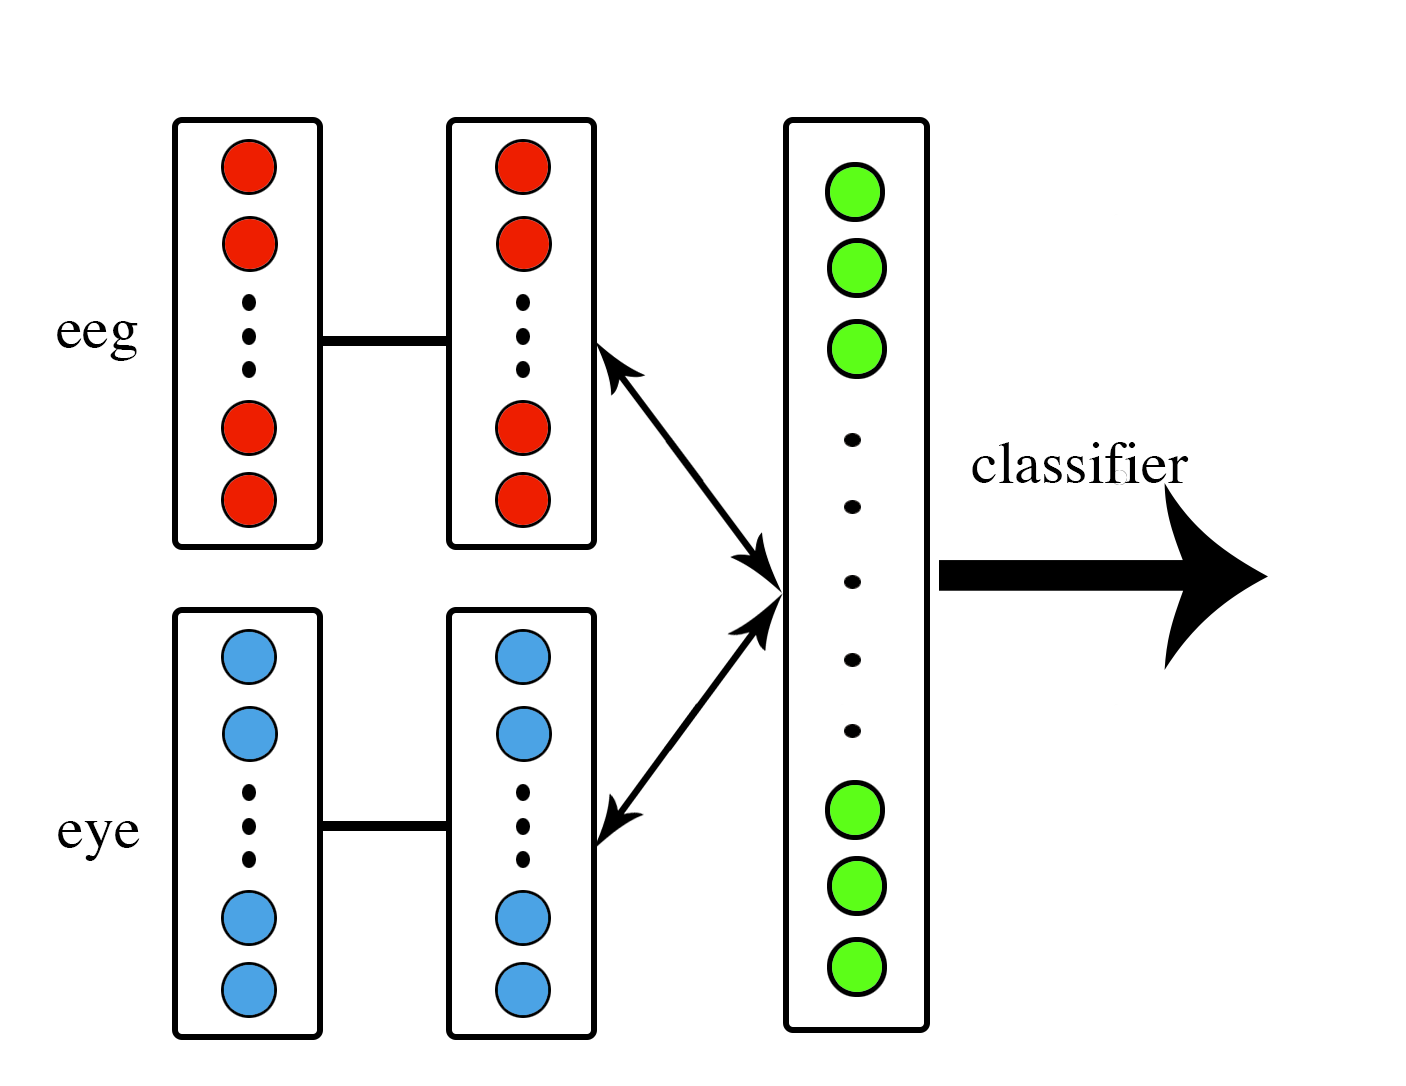
\includegraphics[width=5in]{figure/classify1.png}}
		\centerline{图6-3 算法模型II}
		如上图所示,此算法模型的功能与模型I类似,只是更加复杂,它可以更好的学习到两个模态的数据之间的非线性关系。首先用两个RBM分别提取眼动仪模态和脑电模态的特征,然后再将提取后的特征拼接,并再加一层网络提取共同表达的特征。这个网络一共包含三个RBM,在经过预训练和调参之后,我们获得了比模型I更好的结果。
		
		值得一提的是,模型I与模型II中每个RBM我们尝试了伯努利RBM和高斯RBM,然而在后续工作中我们发现在每个RBM的每个元素中都使用修正线性单元(Rectified Linear Unit,简写为ReLu)替代了sigmoid unit之后,因此这个问题也就无需再考虑,因为不论是从速度还是结果来看,前者都是更优秀的。下文中将对这两个激活函数进行更详尽的对比。
	\subsection{模型III}
		\centerline{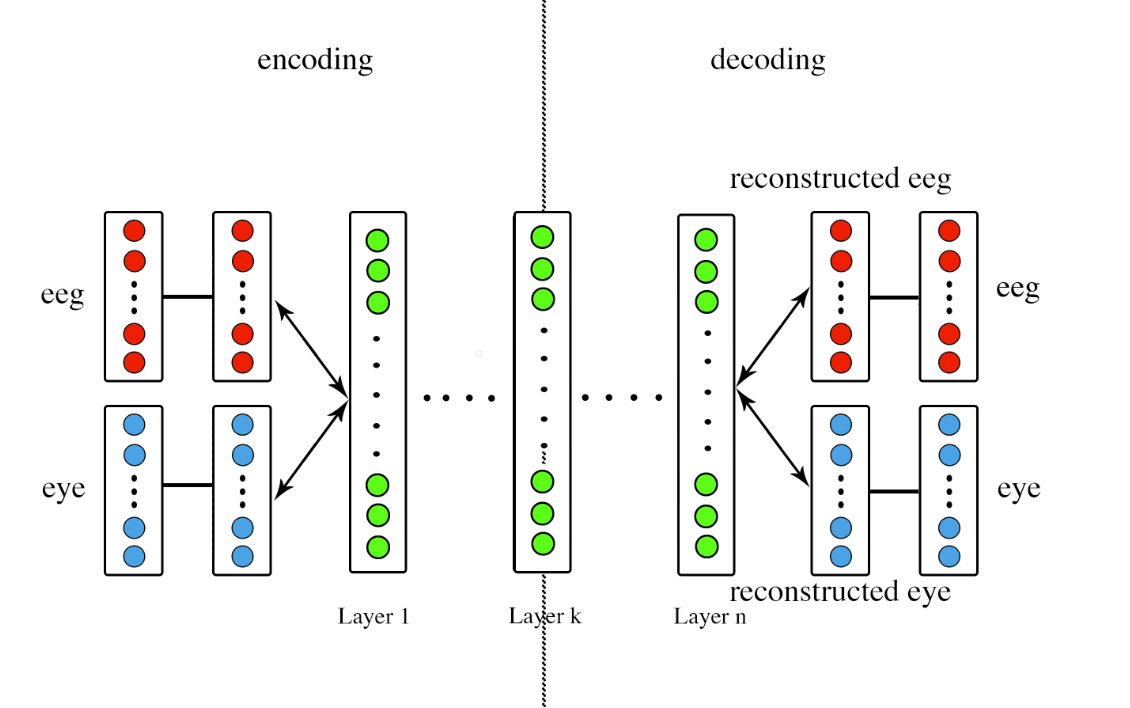
\includegraphics[width=7in]{figure/feature_learning.png}}
		\centerline{图6-4 特征学习模型}
		
		如上图,这就是本文构建的特征提取算法模型。与前两个模型一样,它也接受两个模态的输入,并输出共同特征表达,用于后续的情绪识别任务。
		
		这个算法模型的左边是输入,右边是计算结果。我们把整个特征提取过程的一次迭代分成两个部分,左边半部分是编码过程(encoding),右边半部分是解码过程(decoding)。编码过程和解码过程应该是完全对称的,编码过程是学习更深层次特征的,解码过程是重建数据的。本模型首先分别对两个模态用RBM提取特征,然后对提取后的特征进行拼接,再加上k层网络增加深度来学习两个模态的非线性关系。图片中间的一层是编码的最后一层,也是解码的第一层。整个模型越靠中间的层,深度越深,也就代表了越抽象的特征,越靠近两边的层深度越浅,也就代表了越简单的特征。当计算到最右边一层的重建特征时,我们把整个特征向量一分为二,重新变为脑电数据和眼动仪数据两个模态,然后用输入数据和网络重建的数据进行对比,计算方差来校正整个网络的参数。 注意,即使最左边是数据输入,网络看似越靠右的层有越抽象,越深层次的特征,但是由于我们网络和更新算法的定义,编码过程里面才是越靠右的层越抽象的,而解码过程里面越靠右的层有越具体的特征,因为整个解码过程都在重建原本的特征,所以是不断变的更加具体的。
		
		然而,不像图像识别任务一样,深度网络的每个层次的特征都代表明确的意义,譬如浅层可能是直线和曲线,深层就是复杂的轮廓。趋势是越浅层的越局部越简单,越深层的越广泛越复杂。脑电和眼电数据的深度学习网络里也有相似的道理。为了找出哪个层次的共同特征表达最适用于我们的情绪分类任务,我把从第一层到第n层的共同特征全部提取出来,并进行试验,得到了最终的结果。示意图见下方:
		\centerline{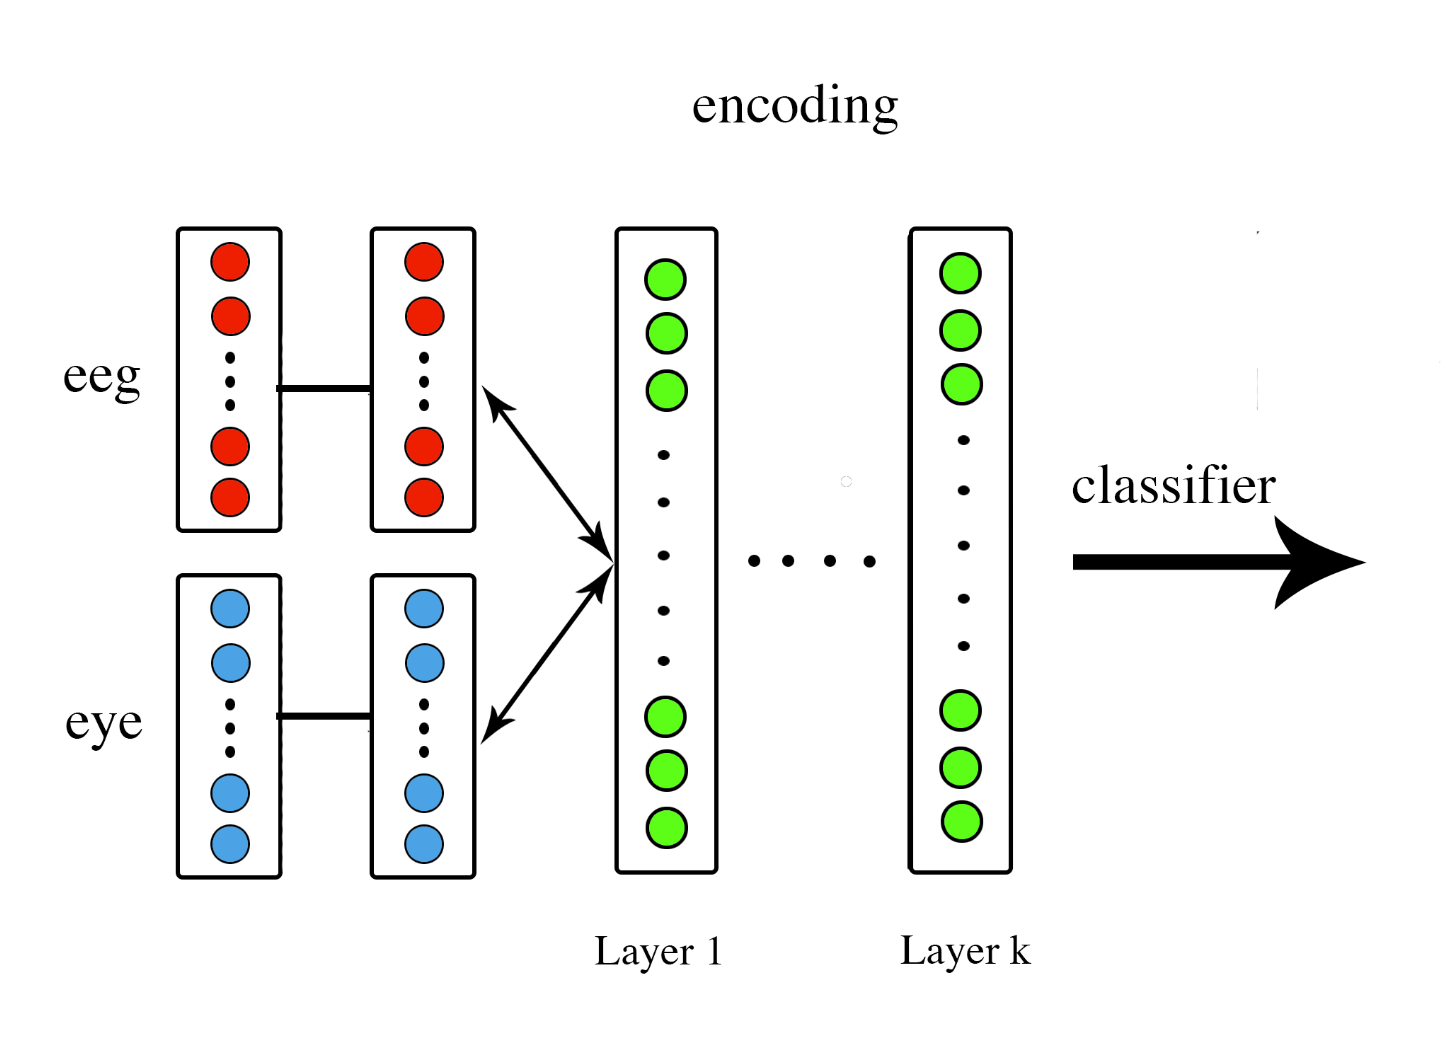
\includegraphics[width=5in]{figure/classifyk.png}}
		\centerline{图6-5 提取在编码阶段的第k层的特征}
		\centerline{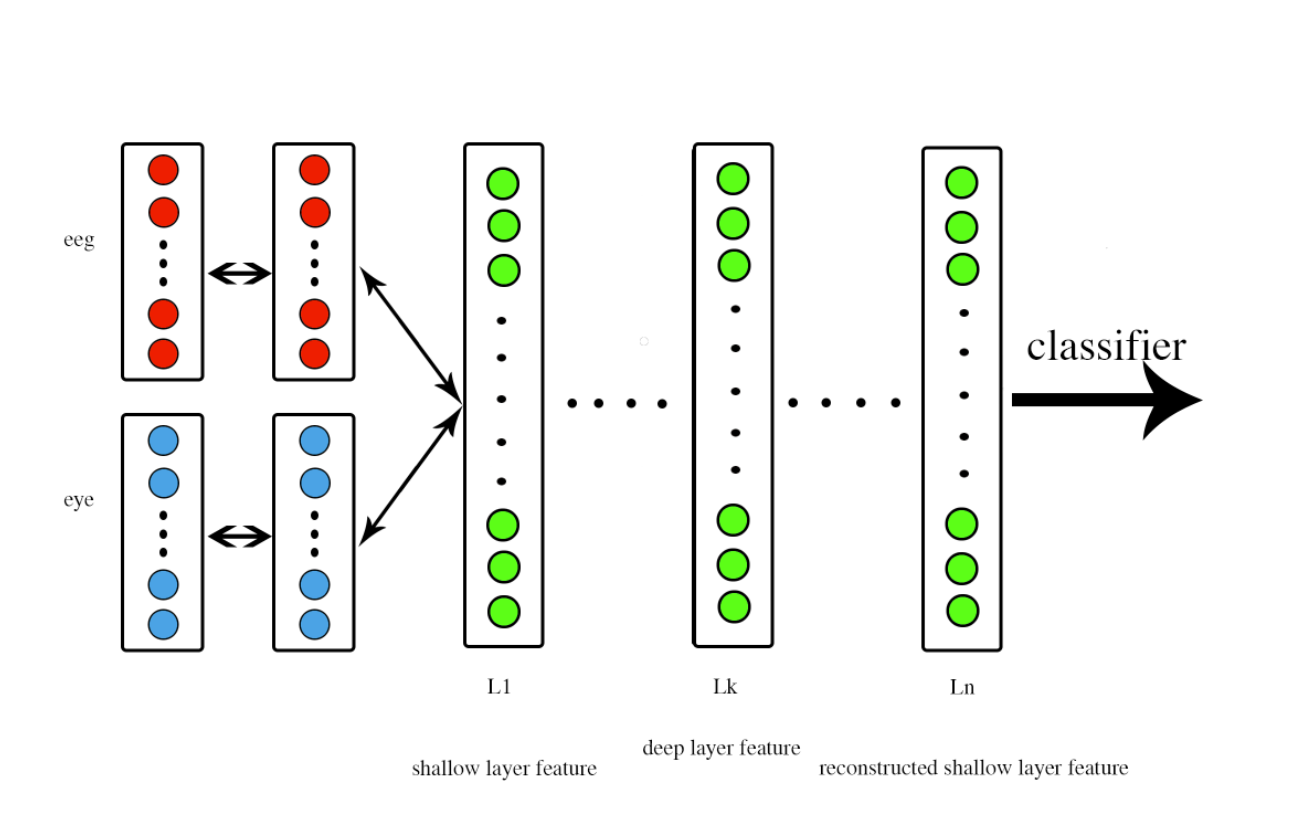
\includegraphics[width=5in]{figure/classifyn.png}}
		\centerline{图6-6 提取在编码阶段的第m层的特征,m为编码阶段最后一层}
		
		\centerline{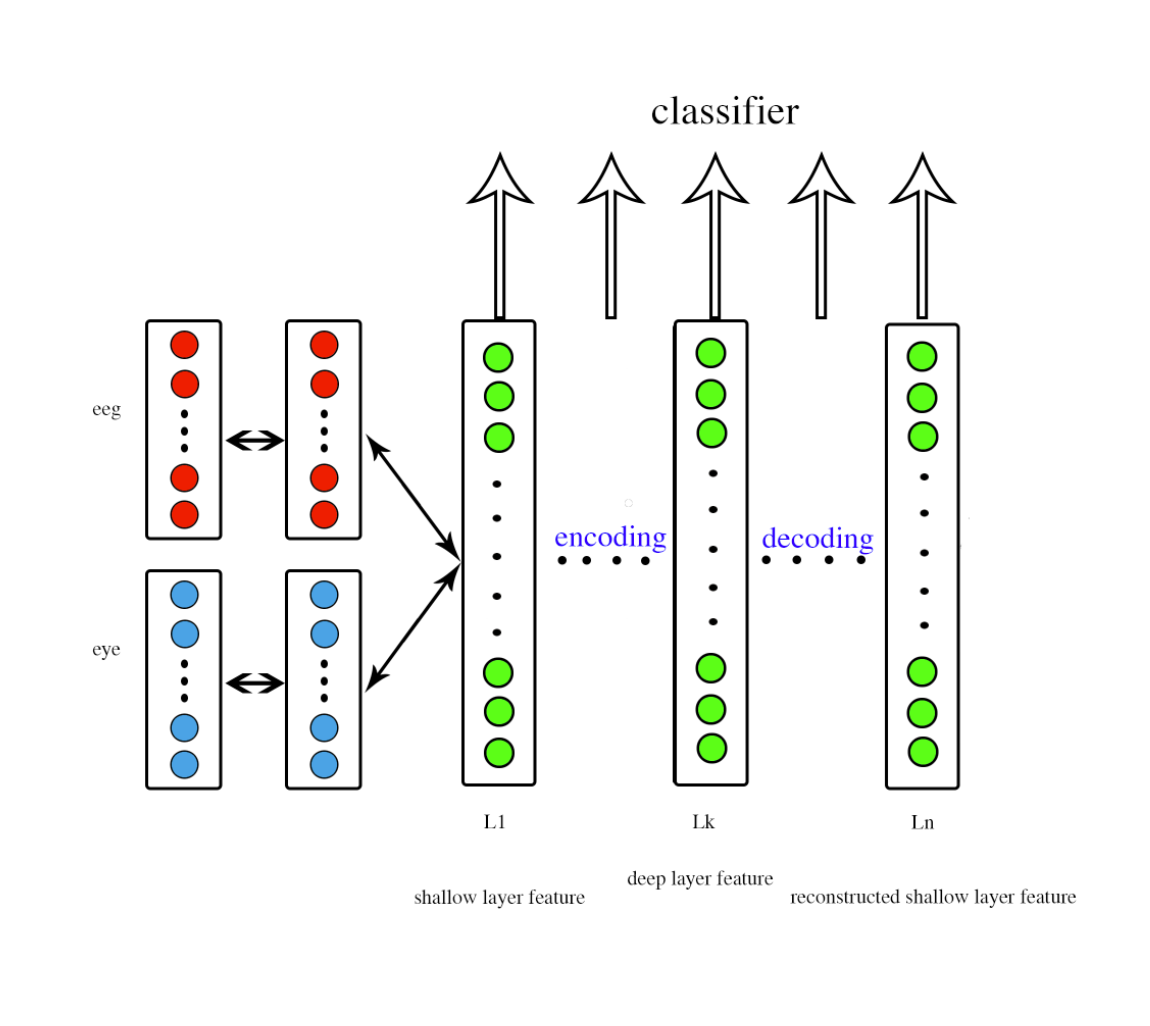
\includegraphics[width=5in]{figure/classify_all.png}}
		\centerline{图6-7 提取所有编码阶段的层次的特征}
		
	\subsection{激励函数的改进}
		
		一直以来,sigmoid函数由于其独特的性质,被广泛的用于神经网络中作为神经元的激励函数。然而最近研究者发现,修正线性单元有成为更加优秀的激励函数的潜力。本论文从理论和实验结果两方面均对这两族函数进行了对比。与线性修正单元近似的一个函数是softplus,两者的定义如下。
		\begin{equation}
		\begin{cases}
		SoftPLus: f(x) = \quad ln(1 + e^x) \\
		ReLu:  f(x) = \quad max(x, 0)
		\end{cases}
		\end{equation}
		
		首先,sigmoid函数一直以来对机器学习的贡献巨大,这是因为它是非线性的激励函数。如果我们不用非线性激励函数,而是直接用$f(x) = x$作为我们的激励函数,那么显而易见,网络的每一层输入都是上一层输出的线性组合,这样一来无论网络有多深,每层有多少个神经元,最终输出总是输入的线性组合,隐藏层就失去了意义,神经网络模型就退化成了最简单的感知机模型。而一旦我们引入sigmoid这样的非线性激励函数,那么每一层就不再是上一层的简单线性组合,而是可以逼近更复杂的函数。并且,sigmoid函数的输出永远在0和1之间,范围确定,很适合作为下一层的输入,哪怕网络十分深,也不会面临指数爆炸等问题。这是神经网络算法的基础。
		
		线性修正单元在2011年被首次提出可以作为一种非线性的激励函数使用在有监督的深度神经网络中,并且它的应用可以避免无监督的预训练。线性修正单元不但具备sigmoid函数的很多优点,还具备更加优秀的性质,可以补偿sigmoid不尽如人意的地方。研究者之所以对线性修正单元投入越来越多的精力,主要有以下几点原因:
		\begin{enumerate}
		\item 采用sigmoid函数的时候,算激活函数时是指数运算,计算量大。
		\item 反向传播求误差梯度时,求导计算量相对大,而采用Relu激活函数,整个过程的计算量节省很多。
		\item 对于深层网络,sigmoid函数反向传播时,很容易就会出现梯度消失(vanishing gradient)的情况,因为每一层都可能会指数减小。
		\item Relu会使一部分神经元的输出为0,这样就造成了网络的稀疏性,并且减少了参数的相互依存关系,避免了过拟合问题(over-fitting)的发生。
		\item Relu函数没有上界,那么前期梯度值可以很大,如此一来训练前期权值可以较大幅度的调整。通过这样来起到加速的效果。
		\item 对于我们的数据来说,如果我们想用sigmoid函数作为激励函数,那么必须要将数据归一化到[0,1]范围内,否则的话我们是在函数的饱和区内,而不在函数剧烈变化的非饱和区内,相当于全部维度都是冗余信息,也就是传播的过程中丢失了大量的信息\upcite{AISTATS2011_GlorotBB11}。而不同归一化结果会产生不同结果,这个冗余的步骤会对结果带来不好的影响。如果用ReLU就解决了这个问题,不再需要进行归一化。
		\item 实验证明,ReLu激活函数可以避免了预训练的流程,节省了训练网络所需要的时间和步骤。
		
		\end{enumerate}
		
		另外,线性修正单元还有一些变种,适用于不同的情况。譬如:
		\begin{itemize}
			\item{
				噪声线性修正单元(Noisy ReLUs)
				
				当线性修正单元被拓展,允许有高斯噪声加入其中后,我们就称它为噪声线性修正单元。 它作为激励函数在计算机视觉领域的应用较为成功。它的函数式如下:
				\begin{align}
				\begin{cases}
					f(x) = max(0, x + Y)\\
					Y \sim \mathcal{N}(0, \sigma (x))
				\end{cases}
				\end{align}
			}
			\\
			\item{
				渗透线性修正单元(Leaky ReLUs)
				
				当所属单元没有被激活的时候,渗透线性修正单元允许产生非零的梯度,它的函数式如下:
				\begin{align}
				f(x) = 
				\begin{cases}
					x & if x > 0 \\
					0.01x & otherwise
				\end{cases}
				\end{align}			
			}
			\item{
				含参线性修正单元(Parametric ReLU)
				
				含参线性修正单元在渗透线性修正单元之上更进一步,它含有接受一个参数a,就像其他的连接权和阈值一样,a也是由神经网络逐渐学习而不断更新的。含参线性修正单元函数式如下:
				\begin{align}
				f(x) = 
				\begin{cases}
					x & if x > 0 \\
					ax & otherwise
				\end{cases}
				\end{align}
			}
		\end{itemize}
		
		
		
		综上所述,线性修正单元作为一种与sigmoid函数相似的函数,虽然它有潜在的问题就是在0处不可导,但是综合来说它可以在复杂的数据集上达到更好的效率和表现。
		
% %# -*- coding: utf-8-unix -*-
\chapter{常见问题}
\label{chap:faq}

{\bfseries{}Q:我是否能够自由使用这份模板?}

A:这份模板以Apache License 2.0开源许可证发布,请遵循许可证规范。

{\bfseries{}Q:我的论文是Word排版的,学校图书馆是不是只收 \LaTeX 排版的论文?}

A:当然不是,Word版论文肯定收。

{\bfseries{}Q:我的论文是 \LaTeX 排版的,学校图书馆是不是只收Word排版的论文?}

A:当然不是,PDF版的电子论文是可以上交的。是否要交Word版就看你导师的喜好了。

{\bfseries{}Q:为什么屏幕上显示的左右页边距不一样?}

A:模板默认是双面打印,迎面页和背面页的页边距是要交换的,多出来的那一部分是留作装订的。

{\bfseries{}Q:为什么在参考文献中会有“//”符号?}

A:那就是国标GBT7714参考文献风格规定的。

{\bfseries{}Q:为什么参考文献中会有[s.n.],[S.l], [EB/OL]等符号?}

A: 那也是国标GBT7714参考文献风格定义的。[s.n.]表示出版者不祥,[S.l]表示出版地不祥,[EB/OL]表示引用的参考文献类型为在线电子文档。

{\bfseries{}Q:如何获得帮助和反馈意见?}

A:你可以通过\href{https://github.com/weijianwen/sjtu-thesis-template-latex/issues}{在github上开issue}
、在\href{https://bbs.sjtu.edu.cn/bbsdoc?board=TeX_LaTeX}{水源LaTeX版}发帖反映你使用过程中遇到的问题。

{\bfseries{}Q:使用文本编辑器查看tex文件时遇到乱码?}

A:请确保你的文本编辑器使用UTF-8编码打开了tex源文件。

{\bfseries{}Q:在CTeX编译模板遇到“rsfs10.tfm already exists”的错误提示?}

A:请删除\verb+X:\CTEX\UserData\fonts\tfm\public\rsfs+下的文件再重新编译。问题讨论见\href{https://bbs.sjtu.edu.cn/bbstcon,board,TeX_LaTeX,reid,1352982719.html}{水源2023号帖}。

{\bfseries{}Q:升级了TeXLive 2012,编译后的文档出现“minus”等字样?}

A:这是xltxtra和fontspec宏包导致的问题。学位论文模板从0.5起使用metatlog宏包代替xltxtra生成 \XeTeX 标志,解决了这个问题。

{\bfseries{}Q:为什么在bib中加入的参考文献,没有在参考文献列表中出现?}

A: bib中的参考文献条目,只有通过\verb+\cite+或者\verb+\upcite+在正文中引用,才会加入到参考文献列表中。

{\bfseries{}Q:在macTex中,为什么pdf图片无法插入?}

A:如果报错是“pdf: image inclusion failed for "./figure/chap2/sjtulogo.pdf".”,则采取以下步骤

\begin{lstlisting}[basicstyle=\small\ttfamily, caption={编译模板}, numbers=none]
  brew install xpdf
  wget http://mirrors.ctan.org/support/epstopdf.zip
  unzip epstopdf.zip
  cp epstopdf/epstopdf.pl /usr/local/bin/
  cd figure/chap2
  pdftops sjtulogo.pdf
  epstopdf sjtulogo.ps
  pdfcrop sjtulogo.pdf
  mv sjtulogo.pdf backup.pdf
  mv sjtulogo-crop.pdf sjtulogo.pdf
\end{lstlisting}

{\bfseries{}Q:如何向你致谢?}

A: 烦请在模板的\href{https://github.com/weijianwen/SJTUThesis}{github主页}点击“Star”,我想粗略统计一下使用学位论文模板的人数,谢谢大家。非常欢迎大家向项目贡献代码。

%# -*- coding: utf-8-unix -*-
%%==================================================
%% chapter06.tex for SJTU Master Thesis
%%==================================================

%\bibliographystyle{sjtu2}%[此处用于每章都生产参考文献]
\chapter{结论与展望}
\label{chap:chap8}
\section{课题结论}{
	本课题主要对脑电信号的的情绪识别进行了研究,为了进一步提高现有的情绪识别结果,我们将多模态深度学习的相关算法应用于该课题上。在前人提出的多模态深度学习算法的基础上,我们又尝试了不同的激励函数和不同深度的网络,最后发现ReLU的结果好于sigmoid,不同深度的特征也有不同的表现,
	
	最终,实验和测试得到的结果比较符合理论的分析和我们的预期,并且相比基准方法和之前的方法有所提高。并且多次实验后,最后选用的库的训练速度较快,训练时间不会很长,令人满意。
}
\section{未来工作展望}

	本课题所提出的算法和各个优化使得最终结果有了提高,然而距离多模态深度学习能够达到的极限还有很大距离。所以,我们根据当前的结果提出了以下有待提高的地方,希望之后的工作中可以参考以下改进意见,继续改进这个算法的性能。
	\begin{enumerate}
		\item 因为前期工作准备时间较长,尝试了多个库,所以导致后期时间较紧,来不及进行调参,包括深度自编码器的参数和分类器的参数,譬如隐层的数目,学习速率,分类器核函数等等。下面如果进行详尽的调参,相信结果一定会有进一步的提高。
		\item 一直以来实验室对结果的比较都是把五个频段的结果分别列出,再列出全频段的结果进行对比。由于实验时间不足,我们只对部分频段的结果进行了实验和分析。未来可以对五个频段进行分别对比,寻找对于这个分类算法的最佳频段。
		\item 现在算法的结果是多模态经过深度网络后融合的分类结果,我们实验结果是直接与不经过任何网络的特征进行对比,这样一来,改变的环境太多。下面如果要通过对比显示多模态于单模态的意义,我们应该对单纯的脑电和眼电分别加上这个算法,用深度自编码器对单模态特征进行特征提取,再对比结果,这样一来改变的只是由单模态到多模态。 而直接把多模态特征拼接,对比我们的多模态深度算法得到的结果,显示的是深度自编码器网络的意义。通过这样的控制变量的方法,我们能进一步说明多模态的意义。
		\item 为了显示我们的深度自编码器学习到的特征更有意义,未来可以写聚类算法分别对原始特征和我们学习到的特征进行对比,自然的,我们学习到的特征会更明显的分为三个类别。通过这样的数据可视化方法可以说明我们学习到了更优秀的特征。
		\item 提取后的特征现在只是用SVM来进行分类,未来可以考虑尝试多个分类器,譬如多层感知机等。
		\item 未来可以进一步实现寻找共同特征表达等任务,即测试和训练所用的数据来自不同模态。
	\end{enumerate}

%% 参考资料
\phantomsection
\addcontentsline{toc}{chapter}{参考文献}
\bibliography{bib/thesis.bib}

\appendix	% 使用英文字母对附录编号,重新定义附录中的公式、图图表编号样式
\renewcommand\theequation{\Alph{chapter}--\arabic{equation}}	
\renewcommand\thefigure{\Alph{chapter}--\arabic{figure}}
\renewcommand\thetable{\Alph{chapter}--\arabic{table}}
\renewcommand\thealgorithm{\Alph{chapter}--\arabic{algorithm}}

%% 附录内容,本科学位论文可以用翻译的文献替代。
%%# -*- coding: utf-8-unix -*-
\chapter{搭建模板编译环境}

\section{安装TeX发行版}

\subsection{Mac OS X}

Mac用户可以从MacTeX主页\footnote{\url{https://tug.org/mactex/}}下载MacTeX 2015。
也可以通过brew包管理器\footnote{\url{http://caskroom.io}}安装MacTeX 2015。

\begin{lstlisting}[basicstyle=\small\ttfamily, numbers=none]
brew cask install mactex
\end{lstlisting}

\subsection{Linux}

建议Linux用户使用TeXLive主页\footnote{\url{https://www.tug.org/texlive/}}的脚本来安装TeXLive 2015。
以下命令将把TeXLive发行版安装到当前用户的家目录下。
若计划安装一个供系统上所有用户使用的TeXLive,请使用root账户操作。

\begin{lstlisting}[basicstyle=\small\ttfamily, numbers=none]
wget http://mirror.ctan.org/systems/texlive/tlnet/install-tl-unx.tar.gz
tar xzvpf install-tl-unx.tar.gz
cd install-tl-20150411/
./install-tl
\end{lstlisting}

\section{安装中文字体}

\subsection{Mac OS X、Deepin}

Mac和Deepin用户双击字体文件即可安装字体。

\subsection{RedHat/CentOS用户}

RedHat/CentOS用户请先将字体文件复制到字体目录下,调用fc-cache刷新缓存后即可在TeXLive中使用新字体。

\begin{lstlisting}[basicstyle=\small\ttfamily, numbers=none]
mkdir ~/.fonts
cp *.ttf ~/.fonts				# 当前用户可用新字体
cp *.ttf /usr/share/fonts/local/	# 所有用户可以使用新字体
fc-cache -f
\end{lstlisting}


%%# -*- coding: utf-8-unix -*-
%% app2.tex for SJTU Master Thesis
%% based on CASthesis
%% modified by wei.jianwen@gmail.com
%% version: 0.3a
%% Encoding: UTF-8
%% last update: Dec 5th, 2010
%%==================================================

\chapter{Maxwell Equations}

选择二维情况,有如下的偏振矢量:
\begin{subequations}
  \begin{eqnarray}
    {\bf E}&=&E_z(r,\theta)\hat{\bf z} \\
    {\bf H}&=&H_r(r,\theta))\hat{ \bf r}+H_\theta(r,\theta)\hat{\bm
      \theta}
  \end{eqnarray}
\end{subequations}
对上式求旋度:
\begin{subequations}
  \begin{eqnarray}
    \nabla\times{\bf E}&=&\frac{1}{r}\frac{\partial E_z}{\partial\theta}{\hat{\bf r}}-\frac{\partial E_z}{\partial r}{\hat{\bm\theta}}\\
    \nabla\times{\bf H}&=&\left[\frac{1}{r}\frac{\partial}{\partial
        r}(rH_\theta)-\frac{1}{r}\frac{\partial
        H_r}{\partial\theta}\right]{\hat{\bf z}}
  \end{eqnarray}
\end{subequations}
因为在柱坐标系下,$\overline{\overline\mu}$是对角的,所以Maxwell方程组中电场$\bf E$的旋度:
\begin{subequations}
  \begin{eqnarray}
    &&\nabla\times{\bf E}=\mathbf{i}\omega{\bf B} \\
    &&\frac{1}{r}\frac{\partial E_z}{\partial\theta}{\hat{\bf
        r}}-\frac{\partial E_z}{\partial
      r}{\hat{\bm\theta}}=\mathbf{i}\omega\mu_rH_r{\hat{\bf r}}+\mathbf{i}\omega\mu_\theta
    H_\theta{\hat{\bm\theta}}
  \end{eqnarray}
\end{subequations}
所以$\bf H$的各个分量可以写为:
\begin{subequations}
  \begin{eqnarray}
    H_r=\frac{1}{\mathbf{i}\omega\mu_r}\frac{1}{r}\frac{\partial
      E_z}{\partial\theta } \\
    H_\theta=-\frac{1}{\mathbf{i}\omega\mu_\theta}\frac{\partial E_z}{\partial r}
  \end{eqnarray}
\end{subequations}
同样地,在柱坐标系下,$\overline{\overline\epsilon}$是对角的,所以Maxwell方程组中磁场$\bf H$的旋度:
\begin{subequations}
  \begin{eqnarray}
    &&\nabla\times{\bf H}=-\mathbf{i}\omega{\bf D}\\
    &&\left[\frac{1}{r}\frac{\partial}{\partial
        r}(rH_\theta)-\frac{1}{r}\frac{\partial
        H_r}{\partial\theta}\right]{\hat{\bf
        z}}=-\mathbf{i}\omega{\overline{\overline\epsilon}}{\bf
      E}=-\mathbf{i}\omega\epsilon_zE_z{\hat{\bf z}} \\
    &&\frac{1}{r}\frac{\partial}{\partial
      r}(rH_\theta)-\frac{1}{r}\frac{\partial
      H_r}{\partial\theta}=-\mathbf{i}\omega\epsilon_zE_z
  \end{eqnarray}
\end{subequations}
由此我们可以得到关于$E_z$的波函数方程:
\begin{eqnarray}
  \frac{1}{\mu_\theta\epsilon_z}\frac{1}{r}\frac{\partial}{\partial r}
  \left(r\frac{\partial E_z}{\partial r}\right)+
  \frac{1}{\mu_r\epsilon_z}\frac{1}{r^2}\frac{\partial^2E_z}{\partial\theta^2}
  +\omega^2 E_z=0
\end{eqnarray}

%%# -*- coding: utf-8-unix -*-
\chapter{从 \CJKLaTeX 转向 \XeTeX }
\label{chap:whydvipdfm}

我习惯把v0.2a使用dvipdfmx编译的硕士学位论文模板称为“ \CJKLaTeX 模板”,而这个使用 \XeTeX 引擎(xelatex程序)处理的模板则被称为“{\XeTeX/\LaTeX}模板”。
从 \CJKLaTeX 模板迁移到{\XeTeX\LaTeX}模板的好处有下:
\begin{enumerate}
\item[\large\smiley] 搭建 \XeTeX 环境比搭建 \CJKLaTeX 环境更容易;
\item[\large\smiley] 更简单的字体控制;
\item[\large\smiley] 完美支持PDF/EPS/PNG/JPG图片,不需要“bound box(.bb)”文件;
\item[\large\smiley] 支持OpenType字体的复杂字型变化功能;
\end{enumerate}

当然,这也是有代价的。由于 \XeTeX 比较新,在我看来,使用 \XeTeX 模板所必须付出的代价是:

\begin{enumerate}
\item[\large\frownie] 必须把你“古老的” \TeX 系统更新为较新的版本。TeXLive 2012和CTeX 2.9.2能够编译这份模板,而更早的版本则无能为力。
\item[\large\frownie] 需要花一些时间把你在老模板上的工作迁移到新模板上。
\end{enumerate}

第一条就看你如何取舍了,新系统通常意味着更好的兼容性,值得升级。而转换模板也不是什么特别困难的事情,可以这样完成:

\begin{enumerate}
\item 备份你要转换的源文件,以防你的工作成果丢失;
\item 将你原来的tex以及bib文件另存为UTF-8编码的文件。iconv、vim、emacs、UEdit等等工具都可以完成。WinEdt对文件编码识别功能很差(到了v6.0还是如此),不推荐作为字符编码转换工具;
\item 将diss.tex导言区中的内容替换为XeTeX模板diss.tex导言区的内容;
\item 将你对原先导言区的修改,小心翼翼地合并到新的导言区中;
\item 使用XeTeX模板中的GBT7714-2005NLang.bst替换原有的bst文件,新的bst文件只是将字符编码转换为UTF-8;
\item 删除bouding box文件;
\item 使用本文\ref{sec:process}介绍的方法,重新编译文档;
\end{enumerate}


%%# -*- coding: utf-8-unix -*-
\chapter{模板更新记录}
\label{chap:updatelog}

\textbf{2015年2月15日} v0.7发布,增加盲审选项,调用外部工具插入扫描件。

\textbf{2015年2月14日} v0.6.5发布,修正一些小问题,缩减git仓库体积,仓库由sjtu-thesis-template-latex更名为SJTUThesis。

\textbf{2014年12月17日} v0.6发布,学士、硕士、博士学位论文模板合并在了一起。

\textbf{2013年5月26日} v0.5.3发布,更正subsubsection格式错误,这个错误导致如"1.1 小结"这样的标题没有被正确加粗。

\textbf{2012年12月27日} v0.5.2发布,更正拼写错误。在diss.tex加入ack.tex。

\textbf{2012年12月21日} v0.5.1发布,在 \LaTeX 命令和中文字符之间留了空格,在Makefile中增加release功能。

\textbf{2012年12月5日} v0.5发布,修改说明文件的措辞,更正Makefile文件,使用metalog宏包替换xltxtra宏包,使用mathtools宏包替换amsmath宏包,移除了所有CJKtilde(\verb+~+)符号。

\textbf{2012年5月30日} v0.4发布,包含交大学士、硕士、博士学位论文模板。模板在\href{https://github.com/weijianwen/sjtu-thesis-template-latex}{github}上管理和更新。

\textbf{2010年12月5日} v0.3a发布,移植到 \XeTeX/\LaTeX 上。

\textbf{2009年12月25日} v0.2a发布,模板由CASthesis改名为sjtumaster。在diss.tex中可以方便地改变正文字号、切换但双面打印。增加了不编号的一章“全文总结”。
添加了可伸缩符号(等号、箭头)的例子,增加了长标题换行的例子。

\textbf{2009年11月20日} v0.1c发布,增加了Linux下使用ctex宏包的注意事项、.bib条目的规范要求,
修正了ctexbook与listings共同使用时的断页错误。

\textbf{2009年11月13日} v0.1b发布,完善了模板使用说明,增加了定理环境、并列子图、三线表格的例子。

\textbf{2009年11月12日} 上海交通大学硕士学位论文 \LaTeX 模板发布,版本0.1a。



\backmatter	% 文后无编号部分 

%% 致谢、发表论文、申请专利、参与项目、简历
%% 用于盲审的论文需隐去致谢、发表论文、申请专利、参与的项目
\makeatletter

%%
% "研究生学位论文送盲审印刷格式的统一要求"
% http://www.gs.sjtu.edu.cn/inform/3/2015/20151120_123928_738.htm

% 盲审删去删去致谢页
%\ifsjtu@review\relax\else
 % %# -*- coding: utf-8-unix -*-
\begin{thanks}

感谢吕宝粮老师在我的实验设计、算法运用以及论文撰写过程中悉心的指导,不仅对我的毕业设计课题提出了了很多宝贵的意见,还培养了我严谨求实的科研态度和大胆创新的科研精神。

感谢刘伟学长在我实验以及算法设计过程给予的无私帮助与指导,特别为我指出了很多深度学习的细节,帮助我快速学习相关算法,并运用到多模态数据上。

感谢各位实验室同学热心的支持我的研究工作, 你们给了我很多宝贵的建议和意想不到的灵感。

感谢电子信息与电气工程学院和计算机科学与工程系为我供优秀的实验设备和实验环境,让我得以完成对情绪识别和多模态深度学习算法的研究。

最后,要感谢我的父母,是你们让我健康长大,一直默默在背后支持我,让我能有机会拥有如此优越的学习条件,谢谢你们一直以来的付出与奉献!

\end{thanks}
 	  %% 致谢
%\fi

\pagestyle{biglast}
\begin{bigabstract}

Emotion plays an important part in the daily life of everyone. Though we could recognize emotions from facial expressions, voice or body movement, with the development of technology and equipment which could collect signals direct from human brains, we are able to recognize emotions with the help of EEG signals. Compared with the original method, EEG signals have a rather direct connection with emotions. Therefore, EEG-based emotion recognition is now the state-of-the-art research area which got the attention of lots of researchers. However, the performance and accuracy are limited if we can access only the single EEG modal.  Now we try to make use of not only the EEG data but the eye motion data, we believe these two data sources can complement each other and thus we can have a better result if we create an algorithm to use them simultaneously. As a result, our algorithm is based on multimodal deep autoencoder, which will be explained below:

	A deep autoencoder is composed of two, symmetrical deep-belief networks that typically have four or five shallow layers representing the encoding half of the net, and second set of four or five layers that make up the decoding half.

	The layers are restricted Boltzmann machines, the building blocks of deep-belief networks, with several peculiarities that we’ll discuss below. Here’s a simplified schema of a deep autoencoder’s structure, which will be  explained below. a deep autoencoder would use binary transformations after each RBM. Deep autoencoders can also be used for other types of datasets with real-valued data, on which you would use Gaussian rectified transformations for the RBMs instead.

	For the encoding process, If, say, the input fed to the network is 784 pixels, then the first layer of the deep autoencoder should have 1000 parameters; i.e. slightly larger.
This may seem counterintuitive, because having more parameters than input is a good way to overfit a neural network.

	In this case, expanding the parameters, and in a sense expanding the features of the input itself, will make the eventual decoding of the autoencoded data possible.
This is due to the representational capacity of sigmoid-belief units, a form of transformation used with each layer. Sigmoid belief units can’t represent as much as information and variance as real-valued data. The expanded first layer is a way of compensating for that.

	The layers will be 1000, 500, 250, 100 nodes wide, respectively, until the end, where the net produces a vector 30 numbers long. This 30-number vector is the last layer of the first half of the deep autoencoder, the pretraining half, and it is the product of a normal RBM, rather than an classification output layer such as Softmax or logistic regression, as you would normally see at the end of a deep-belief network.
For the decoding process, those 30 numbers are an encoded version of the original input data. The second half of a deep autoencoder actually learns how to decode the condensed vector, which becomes the input as it makes its way back.

	The decoding half of a deep autoencoder is a feed-forward net with layers 100, 250, 500 and 1000 nodes wide, respectively. Those layers initially have the same weights as their counterparts in the pretraining net, except that the weights are transposed; i.e. they are not initialized randomly.).

	The decoding half of a deep autoencoder is the part that learns to reconstruct the image. It does so with a second feed-forward net which also conducts back propagation. The back propagation happens through reconstruction entropy.

Deep autoencoder can be used in many cases, as lisited below:
\begin{itemize}
\item Image search

	deep autoencoders are capable of compressing images into 30-number vectors. Image search, therefore, becomes a matter of uploading an image, which the search engine will then compress to 30 numbers, and compare that vector to all the others in its index.Vectors containing similar numbers will be returned for the search query, and translated into their matching image.
\item Data compression

	A more general case of image compression is data compression. Deep autoencoders are useful for semantic hashing, as discussed in this paper by Geoff Hinton
\item .Topic modeling and information retrieval 

	Deep autoencoders are useful in topic modeling, or statistically modeling abstract topics that are distributed across a collection of documents.

	In brief, each document in a collection is converted to a Bag-of-Words (i.e. a set of word counts) and those word counts are scaled to decimals between 0 and 1, which may be thought of as the probability of a word occurring in the doc.
	
	The scaled word counts are then fed into a deep-belief network, a stack of restricted Boltzmann machines, which themselves are just a subset of feedforward-backprop autoencoders. Those deep-belief networks, or DBNs, compress each document to a set of 10 numbers through a series of sigmoid transforms that map it onto the feature space.
	
	Each document’s number set, or vector, is then introduced to the same vector space, and its distance from every other document-vector measured. Roughly speaking, nearby document-vectors fall under the same topic.
	
	For example, one document could be the “question” and others could be the “answers,” a match the software would make using vector-space measurements.
\end{itemize}

	Deep networks have already been successfully applied to unsupervised feature learning for single modalities such as text, images or audio. In this work, we propose a novel application of deep networks to learn features over EEG data and eye motion data. We present multiple algorithm and a series of tasks for multimodal learning and illustrate how to train deep networks that learn features to solve these tasks. In particular, we demonstrate cross modality feature learning, where better features for one modality such as EEG data can be learned if multiple modalities such as EEG data and eye motion data are present at feature learning time. 

	This work focus on the emotion recognition tasks based on the EEG data, to improve the current result of our emotion recognition research, we have applied the multimodal deep learning algorithm containing deep autoencoder to this thesis. With the related multimodal deep learning algorithm created by the researchers, we have tried different activation function and extract feature from different layers. It turned out to be that the rectified linear unit has a better performance than sigmoid function unit while feature from different layer also differs from each other.

	Concretely, 

	However, we see that we are a long way to go before we can make this algorithm really brilliant, so that it can have advantages in both speed and accuracy. So far, what we can see to be done in the future are listed below:
\begin{enumerate}
\item As we tried many libraries before we found this suitable one, we spent a lot of time on it so that we have not enough time to tune the parameters including the number of the hidden units, the learning rate or the core function of our SVM classifier. We believe the result can get better if there is more time for tuning.
\item Our lab usually list the results of five bands(Alpha, Beta, Gamma and so on) and the result of the combination of all five bands respectively for comparison. However, as we don’t have enough time for this work, we just present and analyze the result of the combination of all five bands. We can analyze the five bands respectively to find the best band for this deep autoencoder algorithm.
\item Now the final result represents for the output of multimodal deep autoencoder, and we use this result to compare with the feature that has not been learned or trained by any network, and it is not fair.  In the future, we need to use this algorithm to extract the feature of only EEG data and eye motion data respectively, then use the results to compare with the result of multimodal autoencoder to illustrate the difference between multi-modal and single-modal. Also we need to concatenate the feature of two modals and compare with the result of our algorithm to illustrate the importance of the deep network. Use the method of controlled variable, we can state the advantages of our algorithm clearly.
\item To show that the feature we learned is useful intuitively, we can cluster the learned feature and original feature using K-means cluster algorithm and see the result of the cluster algorithm.
\item Now we just use SVM to classify the feature we learned, we can try different classifier in the future such as multiple perceptron.
\item We can try shared representation task, in which we will use data of one modal to train and data of another modal to test. In this case, the classification can work because the classifier has learned the shared representation of these two modal.
\end{enumerate}

	Finally, the result we get is compatible with the one we anticipated, naturally they are both better than the baseline algorithm. Moreover, after testing so many times, the library we use for the work has a decent speed and can help with the future work.

Furthermore, we expect to show how to learn a shared representation between modalities and evaluate it on a unique task in the future, where the classifier is trained with audio-only data but tested with video-only data and vice-versa. 


%\englishkeywords{\large SJTU, master thesis, XeTeX/LaTeX template}
\end{bigabstract}

]
% 盲审论文中,发表学术论文及参与科研情况等仅以第几作者注明即可,不要出现作者或他人姓名
%\ifsjtu@review\relax
%  %# -*- coding: utf-8-unix -*-

\begin{publications}{99}
    \item\textsc{第一作者}. {中文核心期刊论文}, 2007.  
    \item\textsc{第一作者}. {EI国际会议论文}, 2006.
\end{publications}

%  %# -*- coding: utf-8-unix -*-

\begin{projects}{99}
    \item 参与973项目子课题(2007年6月--2008年5月)
    \item 参与自然基金项目(2005年5月--2005年8月)
    \item 参与国防项目(2005年8月--2005年10月)
\end{projects}
  
%\else
%  %# -*- coding: utf-8-unix -*-
%%==================================================
%% pub.tex for SJTUThesis
%% Encoding: UTF-8
%%==================================================

\begin{publications}{99}
    \item\textsc{Chen H, Chan C~T}. {Acoustic cloaking in three dimensions using acoustic metamaterials}[J]. Applied Physics Letters, 2007, 91:183518.
    \item\textsc{Chen H, Wu B~I, Zhang B}, et al. {Electromagnetic Wave Interactions with a Metamaterial Cloak}[J]. Physical Review Letters, 2007, 99(6):63903.
\end{publications}
	      %% 发表论文
%  %# -*- coding: utf-8-unix -*-
%%==================================================
%% projects.tex for SJTUThesis
%% Encoding: UTF-8
%%==================================================

\begin{projects}{99}
    \item 973项目“XXX”
    \item 自然基金项目“XXX”
    \item 国防项目“XXX”
\end{projects}
  %% 参与的项目
%\fi

% %# -*- coding: utf-8-unix -*-
\begin{patents}{99}
    \item 第一发明人,“永动机”,专利申请号202510149890.0
\end{patents}
	  %% 申请专利
% \include{tex/resume}	  %% 个人简历
\makeatother

\end{document}
